\section{Class F: every switch forward}\label{sec:forward}

The smoothed octagon's period is entirely forward: its word $\ee_2\ee_0\ee_1\ee_2$ advances the
label by one at each of its three switches, and by one more across the twisted seam. This section
shows that no other entirely forward period can be competitive once it has six or more pieces (\cref{thm:class-F}).



The proof plays two consequences of competitiveness against each other. On one side, the Casimir
$\gamma^2$ of the normal multiplier (\cref{def:normal-multiplier}) is a conserved quantity of the
whole period, and a cost at most $\Aoct$ bounds it from above: the frame has to turn through the
angle $\pi/3$ between $g(0)=I$ and $g(T)=R$, and the larger $\gamma^2$ is, the more cost each unit
of turning requires (\cref{prop:fwd-spectral}). On the other side, $\gamma^2$ can be read off at
any piece from the two switch norms on either side of it and their cross pairing
(\cref{lem:gram}). We read it at a piece of smallest active margin. In an all-forward period the
number of pieces satisfies $N\equiv1\pmod 3$, so a period with $N\ge6$ has at least seven pieces,
and its cost is a sum of seven or more edge terms that depend only on consecutive active margins.
At the octagon's margins each edge costs exactly a quarter of $\Aoct$; seven edges fit into the
budget only if the smallest margin is markedly smaller than the octagon's. The switching conditions
at the five pieces around that small margin (stationarity of the cost, and the requirement that the
unused vertex not be preferable at the two outer switches) then hold the two switch norms close to
their least possible value $3/32$. With such norms the Gram identity makes $\gamma^2$ slightly
larger than competitiveness allows. The comparison retains the positive logarithmic correction in the central pairing;
the resulting vertex bounds lie above the spectral cap (\cref{fig:forward}).

We first express the cost through consecutive active margins, then extract the switching
conditions at a minimum. The scalar exclusion reduces those conditions to three residual signs
and a lower bound for the Gram determinant; their proofs occupy
\cref{app:forward-estimates}.

\subsection{The count and the cost of a forward period}

\begin{lemma}\label{lem:fwd-count}
If every switch of a normal vertex period is forward, then $N\equiv1\pmod 3$. In particular
$N\ge6$ implies $N\ge7$.
\end{lemma}

\begin{proof}
The label advances by one at each of the $N$ switches of a period, so $i_N=i_0+N$, while the twist
gives $i_N=i_0+1$ in $\Z/3$ (\cref{lem:sign-sum}).
\end{proof}

At a forward switch from piece $k-1$ to piece $k$ the state has the margins $a_{k-1}$ and $a_k$ for
the labels $i_{k-1}$ and $i_k$, and the relation $p_0p_1+p_1p_2+p_2p_0=4$ (\cref{lem:margins})
determines the third margin, $(4-a_{k-1}a_k)/(a_{k-1}+a_k)$. Its positivity and the one-arc formula
(\cref{lem:one-arc}) on piece $k$ give the following.

\begin{lemma}\label{lem:fwd-cycle}
In a normal vertex period with every switch forward, for every $k$,
\[
a_{k-1}a_k<4,\qquad
q_k=\frac{(a_{k-1}+a_k)(a_k+a_{k+1})}{a_k^2+4}>1,
\]
and the cost is
\begin{equation}\label{eq:fwd-cost}
\cost=\frac{\sqrt3}{4}\sum_{j=0}^{N-1}G(a_j,a_{j+1}),
\end{equation}
where
\[
G(a,b)=3ab-4-(a^2+b^2)\log(a+b)+\tfrac12a^2\log(a^2+4)+\tfrac12b^2\log(b^2+4).
\]
\end{lemma}

So in a forward period the durations are determined by the active margins, and
\eqref{eq:fwd-cost} expresses the cost through the margins alone. The function $G$ is the signed
action of \cref{lem:per-signed-action} with all signs positive.
The arc costs of \cref{lem:one-arc} differ from the terms of \eqref{eq:fwd-cost} by a telescoping
sum, which vanishes over a period. For the octagon, $N=4$ and all four active margins equal $a$ with
$a^2=4/(2\sqrt2-1)$; then $(a^2+4)/(4a^2)=1/\sqrt2$, so
$G(a,a)=3a^2-4+a^2\log\frac{a^2+4}{4a^2}=2\doct$ and the four edges cost
$\sqrt3\,G(a,a)=\Aoct$.

\Cref{app:fwd-edge} collects the properties of $G$ that we use: $G$ is symmetric, increasing in
each argument as long as $ab\le8$, has positive mixed derivative
$\partial_a\partial_bG=2(a^2+ab+b^2)/(a+b)^2$, and satisfies $G(a,a)\ge0$ when $a^2\ge4/3$.

\subsection{The window at a minimum}

Fix a piece $m$ whose active margin $a=a_m$ is the least of all active margins of the period, and
write
\[
(p,b,a,c,d)=(a_{m-2},a_{m-1},a_m,a_{m+1},a_{m+2})
\]
for the active margins of the five pieces around it; all are at least $a$. Lowering every active
margin outside this window to $a$ lowers each edge term of \eqref{eq:fwd-cost}, by monotonicity of
$G$, and keeps the two edges $G(a,p)$ and $G(d,a)$ that close the window.

\begin{lemma}[The seven-entry bound]\label{lem:fwd-seven}
If $N\ge7$, there is an integer $n\ge0$ with
\begin{multline*}
G(a,p)+G(p,b)+G(b,a)+G(a,c)+G(c,d)+G(d,a)+(n+1)\,G(a,a)\\
\le\sum_{j=0}^{N-1}G(a_j,a_{j+1})=\frac{4}{\sqrt3}\,\cost .
\end{multline*}
\end{lemma}

The window is described by dimensionless quantities. Put
\begin{gather*}
\nu=\frac4{a^2},\qquad z=\frac ba,\qquad w=\frac ca,\qquad \hat p=\frac pa,\qquad \hat d=\frac da,\\
\hat s_-=1+z,\quad\ \hat s_+=1+w,\quad\ \hat K=1+\nu,\quad\ \hat K_-=z^2+\nu,\quad\ \hat K_+=w^2+\nu,
\end{gather*}
so that $\hat s_-=s_{m-1}/a$, $\hat s_+=s_m/a$, and $\hat K,\hat K_-,\hat K_+$ are
$K_m,K_{m-1},K_{m+1}$ divided by $a^2$. These letters are local to this section and to
\cref{app:forward-estimates}. The factors of the three central pieces are
\[
h:=q_{m-1}=\frac{(\hat p+z)\hat s_-}{\hat K_-},\qquad
q:=q_m=\frac{\hat s_-\hat s_+}{\hat K},\qquad
k:=q_{m+1}=\frac{(w+\hat d)\hat s_+}{\hat K_+}.
\]
Minimality gives $\hat p,z,w,\hat d\ge1$, and the products $pb,ab,ac,cd<4$ of
\cref{lem:fwd-cycle} read $\hat pz<\nu$, $z<\nu$, $w<\nu$, $w\hat d<\nu$. Together these give
\begin{equation}\label{eq:fwd-factor-range}
\frac{\hat s_-^2}{\hat K_-}\le h\le\frac{\hat s_-}{z},\qquad
\frac{\hat s_+^2}{\hat K_+}\le k\le\frac{\hat s_+}{w}.
\end{equation}

\subsection{The normal multiplier at the window}

The costate enters through three numbers: eight times the switch norms on either side of the
central piece, and sixteen times the cross pairing on it (\cref{def:normal-multiplier}),
\[
u:=8d_{m-1},\qquad v:=8d_m,\qquad E:=16e_m .
\]
(The letter $u$ does not denote the control here.) At a forward switch the switch norm is at least
$j/2\ge3/32$ (\cref{lem:switch-norms}), so $u,v\ge3/4$; the proof will show that $u$ and $v$ exceed
$3/4$ only by little.

Three facts about $(u,v,E)$ come from the Pontryagin conditions. First, stationarity
(\cref{lem:stationarity}) at the piece $m$ gives one linear relation, and at the pieces $m\mp1$,
after the coordinates of the multiplier are transported across the pieces $m$ and $m+1$
(\cref{def:normal-multiplier}), two more. Second, at the forward switch from piece $m-2$ into piece
$m-1$ the vertices of the two pieces tie, and the third vertex, which neither piece uses, may not do
better (\cref{lem:vertex-hamiltonians}): its switching function is $\chi=-4\sqrt3\,G_L/(p+b)^2\le0$
for an affine expression $G_L$ in the entries of the multiplier. Read in the frame of the piece
$m-1$, the inequality $G_L\ge0$ is a lower bound for $u$ in terms of the exterior factor $h$ and the
ratio $z$; the switch from $m+1$ into $m+2$ gives the same kind of bound for $v$. Third, the Gram
identity (\cref{lem:gram}) at the doubly forward piece $m$ expresses the Casimir.

\begin{proposition}[The window data]\label{prop:fwd-window}
In the setting above, put
\begin{align*}
A&=1+z+w-\frac1{\hat s_-}-\frac1{\hat s_+}+\frac1{\hat K}-\log q,\\
B&=\frac{\hat K_-h}{\hat s_-}+1-\frac{z^2\hat s_-}{\hat K_-h}-\frac{z^2}{\hat s_-}
   +\frac{z^3}{\hat K_-}-z\log h,\\
\eta&=\frac{\hat K(h\hat s_--z)}{\hat K_-},\qquad
n_1=\frac{\hat s_-^2(\nu-z)(h-1)}{\hat K_-},\\
n_2&=\frac{\hat K^2}{\hat s_-\hat K_-}\bigl(q-1+(h-1)(q\hat s_--1)\bigr),
\end{align*}
and let $F_x(r)=1+x^2r-xr\log r/(r-1)$ for $r>1$. Then:
\begin{enumerate}
\item (central row) $\hat s_-u+\hat s_+v-E=A$;
\item (left row) $n_1u+n_2v=\eta A-B$, and the right row is obtained by exchanging
  $(z,\hat p,h,u)$ with $(w,\hat d,k,v)$;
\item (exterior floors) $u\ge F_{z/\hat s_-}(h)$ and $v\ge F_{w/\hat s_+}(k)$;
\item (Gram identity) $\gamma^2=\hat K^2(4uv-E^2)/(16\nu^2)$, and $\gamma^2=\det\Lambda_1(0)/12$.
\end{enumerate}
\end{proposition}

In physical units the central row reads $(a+b)u+(a+c)v-aE=\frac12\partial_{a_m}\sum_jG(a_j,a_{j+1})$:
it is the stationarity of the cost \eqref{eq:fwd-cost} in the central margin. For $x\ge1/2$ the
floor $F_x(r)$ increases in $r$ and tends to $1-x+x^2\ge3/4$ as $r\to1$. The floor for $u$ is the
missing-control inequality: once the stationarity of piece $m-1$ is used, $G_L$ is a positive multiple of
$u-F_{z/\hat s_-}(h)$.

\subsection{The competitive cap}

\Cref{prop:cost-casimir} bounds the cost below by a function of the Casimir. Case F uses the
following sharper bound; since $(\kappa+\frac32)(2\kappa+3)-12\kappa=2(\kappa-\frac32)^2\ge0$, it
implies $\cost\ge4\pi\kappa/(2\kappa+3)$.

\begin{proposition}[Spectral cost--Casimir bound]\label{prop:fwd-spectral}
Let $P$ be a normal vertex period with every switch forward. Then $\det\Lambda_1(0)>0$, and with
$\kappa=\sqrt{\det\Lambda_1(0)}$,
\[
\cost\ge\frac\pi3\Bigl(\kappa+\frac32\Bigr).
\]
\end{proposition}

\begin{proof}
The Casimir is positive by the projective argument of \cref{prop:ellipticity}: at each doubly
forward piece the projective coordinate of the switch vectors increases strictly, so over a period
the increments cannot add up to zero. With one
positive switch norm this makes $\Lambda_1(0)$ negative elliptic, $\Lambda_1(0)=-\kappa\,hJh^{-1}$
for some $h\in\SLtwo$. Put $B(t)=h^{-1}g(t)$; then $B'=BX$ and $B(T)=B(0)R$. Write
$\rho=-\frac12\tr(JX)$ and $\rho_R=-\frac12\tr(JBXB^{-1})$, so that the cost density is $3\rho$, and
let $z_B=\frac12(B_{00}+B_{11})+\frac i2(B_{10}-B_{01})$ be the rotation coordinate of $B$.
Conservation, $\Lambda_1(t)=g(t)^{-1}\Lambda_1(0)g(t)$, gives $\tr(\Lambda_1X)=2\kappa\rho_R$, and
the vertex Hamiltonians being nonpositive gives $\tr\bigl((\Lambda_1+\frac32J)X\bigr)\le0$, that
is, $2\kappa\rho_R\le3\rho$. The polar angle $\theta$ of $z_B$ changes at the rate
$\theta'=(\rho+\rho_R)/(2\abs{z_B}^2)>0$ and turns through at least $\pi/3$, since $B(T)=B(0)R$.
To prove the pointwise inequality
\begin{equation}\label{eq:fwd-spectral-key}
  (\rho+\rho_R)^2\le4\abs{z_B}^2\rho\rho_R,
\end{equation}
use the singular value decomposition $B=U\operatorname{diag}(\ell,\ell^{-1})V$ with $U,V$
rotations and $\ell\ge1$. Rotations preserve $\rho$ and $\abs{z_B}$, so replace $X$ by
$VXV^{-1}=\begin{psmallmatrix}a&-\rho-d\\ \rho-d&-a\end{psmallmatrix}$. Since $\det X=1$,
$\rho^2-d^2=1+a^2$. With $c=(\ell^2+\ell^{-2})/2$ and $s=(\ell^2-\ell^{-2})/2$, one has
$\rho_R=c\rho+sd$, $4\abs{z_B}^2=2(c+1)$ and $c^2-s^2=1$. Consequently
\[
  4\abs{z_B}^2\rho\rho_R-(\rho+\rho_R)^2
  =s^2(\rho^2-d^2)=s^2(1+a^2)\ge0.
\]
Thus
\begin{equation}\label{eq:fwd-spectral-pointwise}
  0<\theta'=\frac{\rho+\rho_R}{2\abs{z_B}^2}
  \le\frac{2\rho\rho_R}{\rho+\rho_R}
  \le\frac{6\rho}{2\kappa+3}.
\end{equation}
Integrating,
$\pi/3\le2\cost/(2\kappa+3)$.
\end{proof}

Once negative ellipticity is known, this pointwise argument does not use the switch signs.
In particular, on every subinterval $[s,t]\subseteq[0,T]$ it gives
\begin{equation}\label{eq:spectral-subinterval}
  \Bigl(\kappa+\frac32\Bigr)\bigl(\theta(t)-\theta(s)\bigr)
  \le-\frac32\int_s^t\tr(JX(r))\,\dd r.
\end{equation}
For a competitive period the total angle is exactly $\pi/3$: it is positive, congruent to
$\pi/3$ modulo $2\pi$, and at most $\Aoct/(\kappa+3/2)<2\pi/3$.
In the twisted extension the cost density and $\theta'$ are $T$-periodic: conjugation by $R$
preserves $\tr(JX)$, while $B(t+T)=B(t)R$ multiplies $z_B$ by $e^{i\pi/3}$.
Splitting an interval at period endpoints therefore extends \eqref{eq:spectral-subinterval}
to intervals in $\R$.
The interval form will allow a bridge to be charged its exact cost while the complement is
charged by its angle (\cref{eq:ss-defect}).

\begin{corollary}[Competitive cap]\label{cor:fwd-cap}
A competitive normal vertex period with every switch forward has
\[
 \gamma^2\le\Gamma_{\rm oct}:=
 \frac1{12}\left(\frac{3\Aoct}{\pi}-\frac32\right)^2
 <\frac{9193}{50000}.
\]
\end{corollary}

\begin{proof}
The exact bound follows from \cref{prop:fwd-spectral} and $\cost\le\Aoct$.
By \cref{lem:octagon-cost-comparison},
\[
 \frac{3\Aoct}{\pi}-\frac32<\frac{101}{68},\qquad
 \Gamma_{\rm oct}<\frac1{12}\left(\frac{101}{68}\right)^2
 <\frac{9193}{50000}.
\]
This is also the cap used for mixed periods in \cref{lem:m2-casimir}.
\end{proof}

\subsection{The scalar exclusion}

From now on suppose $N\ge6$, so $N\ge7$ by \cref{lem:fwd-count}. The window data of
\cref{lem:fwd-seven,prop:fwd-window}, the bounds \eqref{eq:fwd-factor-range} and the cap
$\gamma^2<9193/50000$ are finitely many real equations and inequalities. We show that they are
inconsistent. The data are symmetric under the
exchange of the two sides, which exchanges the left and right rows and the two floors, so we may
assume $z\le w$. The steps follow; \cref{app:forward-estimates} proves the scalar inequalities.

\runin{Step 1: the minimum is not small.} The first restriction does not use the cost.

\begin{lemma}[Small forward minimum]\label{lem:fwd-small}
$\nu<3$, that is, $a^2>4/3$.
\end{lemma}

If $\nu\ge3$, the left row and the floors force the residual
$\eta A-B-n_1F_{z/\hat s_-}(h)-n_2V$ to be nonnegative, where $V$ is the floor for $v$ evaluated at
the smallest factor that minimality allows. \Cref{app:fwd-small} shows that this residual is
negative: lowering the larger neighbour $w$ does not decrease it, which leaves three faces, and on
each face the residual is a function of $h$ with explicit value and slope at $h=1$ and a controlled
second derivative.

\runin{Step 2: the minimum is below the octagon's scale.} Since $a^2>4/3$, $G(a,a)\ge0$, so the
seven-entry bound holds with $n=0$. If $a^2\ge20/11$, each of the seven edges is at least
$G(a_0,a_0)$ with $a_0^2=20/11$, and $G(a_0,a_0)=\frac{20}{11}\bigl(\frac45-\log\frac54\bigr)\ge
\frac{23}{22}$, so the cost would exceed $161\sqrt3/88>29\sqrt3/16>\Aoct$.
The last comparison follows from the midpoint logarithm bound in \cref{app:fwd-budget}.

\begin{lemma}\label{lem:fwd-threshold}
$11/5<\nu<3$.
\end{lemma}

\runin{Step 3: the exterior budget.} The rectangle inequality
$G(x,y)\ge G(x,a)+G(a,y)-G(a,a)$ for $x,y\ge a$, applied to the edges $(p,b)$ and $(c,d)$, turns
the seven-entry bound into
\[
\frac{\sqrt3}{\nu}\bigl(2g_\nu(\hat p)+2g_\nu(z)+2g_\nu(w)+2g_\nu(\hat d)-g_\nu(1)\bigr)\le\Aoct,
\qquad g_\nu(x)=\frac{G(a,ax)}{a^2}.
\]
On $[1,\nu]$ the function $g_\nu$ is increasing and concave, so for a given sum
$\hat p+z+w+\hat d$ the left side is smallest when the excess over four is carried by one ratio. The
joint concavity argument of \cref{app:fwd-budget} then gives:

\begin{lemma}[Exterior budget]\label{lem:fwd-budget}
$\hat p+z+w+\hat d<(5\nu+1)/3$. Consequently $z+w<5(\nu-1)/3$ and
$h\le\hat s_-(5\nu-2-3w)/(3\hat K_-)$.
\end{lemma}

The bound on $h$ follows from $h\hat K_-/\hat s_-=\hat p+z$ and $k\hat K_+/\hat s_+=\hat d+w\ge
\hat s_+$.

\runin{Step 4: the larger neighbour.} The floors and the left row give
$\eta A-B=n_1u+n_2v\ge n_1F_{z/\hat s_-}(h)+n_2F_{w/\hat s_+}(\hat s_+^2/\hat K_+)$, since
$n_2\ge n_1\ge0$, the floor increases in the factor and $k\ge\hat s_+^2/\hat K_+$. The difference of
the two sides is a residual $\mathcal E_N$, and $\mathcal E_N<0$ whenever $w\ge4/3$
(\cref{app:fwd-signs}).

\begin{lemma}[Neighbour bound]\label{lem:fwd-neighbour}
If $z\le w$, then $w<4/3$.
\end{lemma}

\runin{Step 5: the switch norms are nearly minimal.} Write $u=\frac34+\delta u$ and
$v=\frac34+\delta v$. The floors become $\delta u\ge L(z,h)\ge0$ and
$\delta v\ge L(w,\hat s_+^2/\hat K_+)\ge0$ for an explicit function $L$ (\cref{app:fwd-centered}),
and the left row becomes the centered identity
\begin{equation}\label{eq:fwd-centered}
n_1\,\delta u+n_2\,\delta v=r,\qquad r:=\eta A-B-\tfrac34(n_1+n_2),
\end{equation}
with $n_2>n_1\ge0$. If $\delta u+\delta v\ge1/32$, then \eqref{eq:fwd-centered}, written as
$r=n_1(\delta u+\delta v)+(n_2-n_1)\delta v$, and the floor for $\delta v$ give
\[
\mathcal E_\Sigma:=r-\frac{n_1}{32}-(n_2-n_1)\,L\Bigl(w,\frac{\hat s_+^2}{\hat K_+}\Bigr)\ge0;
\]
if $\delta v\ge1/64$, they give $\mathcal E_v:=r-n_1L(z,h)-n_2/64\ge0$. Neither residual decreases
when $w$ is lowered to $z$. On the resulting symmetric domain,
$\mathcal E_v<0$ by \cref{lem:fwd-individual}; the sum residual is negative by \cref{lem:fwd-sum}.

\begin{lemma}[Norm bounds]\label{lem:fwd-norms}
If $z\le w$, then $\delta u,\delta v\ge0$, $\delta u+\delta v<1/32$ and $\delta v<1/64$.
\end{lemma}

\runin{Step 6: the Casimir is too large.} The central row and the identity
$\frac34(\hat s_-+\hat s_+)-A=e_0-\varphi$, where
\[
e_0=1-\frac{\hat K}8+\frac1{\hat K},\quad
\varphi=f\Bigl(\frac{\hat s_-}2\Bigr)+f\Bigl(\frac{\hat s_+}2\Bigr)+f\Bigl(\frac4{\hat K}\Bigr),
\quad f(r)=\frac{r-r^{-1}}2-\log r,
\]
give $E=e_0-\varphi+\hat s_-\delta u+\hat s_+\delta v$, with $0\le\varphi<e_0$ by the
integral bound in \cref{app:fwd-casimir}. Substituted into the Gram identity, the norm bounds give:

\begin{lemma}[Conditional Casimir bound]\label{lem:fwd-casimir}
Let $11/5\le\nu<3$, $1\le z\le w\le4/3$, $z+w\le5(\nu-1)/3$, $\delta u,\delta v\ge0$,
$\delta u+\delta v\le1/32$, $\delta v\le1/64$ and
$E=e_0-\varphi+\hat s_-\delta u+\hat s_+\delta v$. Then
\[
\frac{\hat K^2\bigl(4(\frac34+\delta u)(\frac34+\delta v)-E^2\bigr)}{16\nu^2}>\frac{9193}{50000}.
\]
\end{lemma}

\begin{proof}[Proof of \cref{thm:class-F}]
Suppose $P$ is competitive and all-forward, with $N\ge6$. By \cref{lem:fwd-count} $N\ge7$; take the
window at a global minimum of the active margins. Its data satisfy
\cref{lem:fwd-seven,prop:fwd-window} and \cref{cor:fwd-cap}; after exchanging the two sides if
necessary, $z\le w$. \Cref{lem:fwd-threshold,lem:fwd-budget,lem:fwd-neighbour,lem:fwd-norms} give
the hypotheses of \cref{lem:fwd-casimir}, which together with the Gram identity gives
$\gamma^2>9193/50000$, contradicting \cref{cor:fwd-cap}.
\end{proof}

\begin{figure}[htbp]
\centering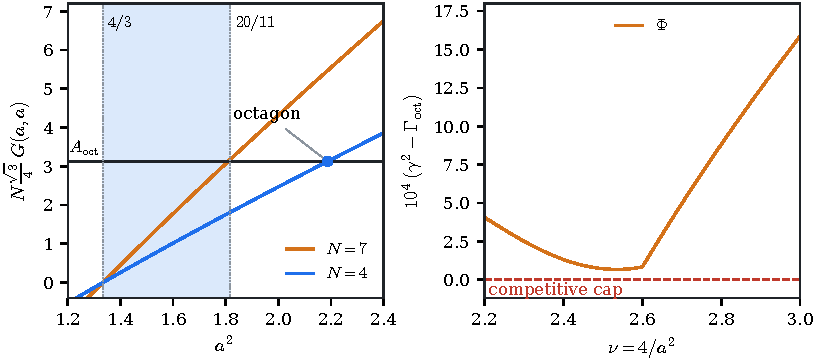
\includegraphics[width=\textwidth]{figures/fig-forward-window.pdf}
\caption{The two sides of the case F contradiction. Left: the cost $N\frac{\sqrt3}4G(a,a)$ of $N$
equal edges against $a^2$, for $N=4$ and $N=7$. Four edges at the octagon's margin cost exactly
$\Aoct$ (dot). Seven edges cost more than $\Aoct$ once $a^2\ge20/11$ (\cref{lem:fwd-threshold}),
and $a^2>4/3$ by \cref{lem:fwd-small}, so the least active margin of a long competitive forward
period lies in the shaded band. Right: on that band, under the bounds of
\cref{lem:fwd-budget,lem:fwd-neighbour,lem:fwd-norms}, the proof uses the scalar curve $\Phi$ of
\cref{app:fwd-casimir}. This curve bounds the Casimir at the two vertices on the norm-sum edge;
the other two vertices are estimated separately in the proof.
The curve is strictly convex up to the shape ceiling $\nu=13/5$
and increases thereafter. Its minimum lies above the competitive cap
$\Gamma_{\rm oct}$ (dashed), defined in \cref{cor:fwd-cap}.
The vertical scale is $10^{4}(\gamma^2-\Gamma_{\rm oct})$.}\label{fig:forward}
\end{figure}

\subsection{Estimates for class F}\label{app:forward-estimates}

This subsection proves the scalar inequalities of \cref{sec:forward}, in its notation: $\nu=4/a^2$,
the ratios $z,w,\hat p,\hat d\ge1$, $\hat s_\pm$, $\hat K$, $\hat K_\pm$, the factors $h,q,k$, the
row coefficients $A,B,\eta,n_1,n_2$ and the floor $F_x(r)$ of \cref{prop:fwd-window}. Throughout,
\[
f(r)=\frac{r-r^{-1}}2-\log r,\qquad \beta(y)=\frac{y^2+y+1}{(1+y)^2}=1-\frac1{1+y}+\frac1{(1+y)^2},
\]
so that $\beta(w)$ is the value $1-x+x^2$ of the floor $F_x$ at $r=1$ for $x=w/(1+w)$.

\subsubsection{The edge function}\label{app:fwd-edge}

Let $G$ be the edge function of \eqref{eq:fwd-cost}. Its partial derivatives are
\begin{align*}
\partial_bG(a,b)&=3a-2b\log(a+b)-\frac{a^2+b^2}{a+b}+b\log(b^2+4)+\frac{b^3}{b^2+4},\\
\partial_a\partial_bG(a,b)&=\frac{2(a^2+ab+b^2)}{(a+b)^2},\qquad
\partial_a\partial_b^2G(a,b)=\frac{2a(b-a)}{(a+b)^3}.
\end{align*}
\begin{enumerate}
\item (Monotonicity) The bound $\log y\ge1-1/y$ at $y=(b^2+4)/(a+b)^2$ gives
  $\partial_bG(a,b)\ge a(a+2b)(b^2-ab+8)/\bigl((a+b)(b^2+4)\bigr)$, which is positive when
  $ab\le8$. So $G$ increases in each argument while the product of its arguments is at most $8$.
  All products of consecutive active margins are below $4$.
\item (Rectangle inequality) Since $\partial_bG(x,\cdot)-\partial_bG(a,\cdot)\ge0$ for $x\ge a$,
  integrating in the second variable gives $G(x,y)\ge G(x,a)+G(a,y)-G(a,a)$ for $x,y\ge a>0$.
\item (Concavity) If $a^2\ge4/3$, then $G(a,\cdot)$ is concave on $[a,4/a]$. Since
  $\partial_a\partial_b^2G\ge0$ for $a\le b$, it suffices to check $\partial_b^2G<0$ at $a=b$ when
  $4/3\le b^2\le4$, and at $a=4/b$. With $\varsigma=4b^2/(b^2+4)\in[1,2]$ one has
  $\partial_b^2G(b,b)=-\log\varsigma-\frac32+\frac54\varsigma-\frac18\varsigma^2$, which increases in
  $\varsigma$ (its derivative is $(\varsigma-1)(4-\varsigma)/(4\varsigma)$) up to the value
  $\frac12-\log2<0$ at $\varsigma=2$; and $\partial_b^2G(4/b,b)=\log\varrho+1-\varrho<0$ with
  $\varrho=b^2/(b^2+4)$.
\item (Scaling) $G(ax,ay)=a^2g_\nu(x,y)$ with
  $g_\nu(x,y)=3xy-\nu-(x^2+y^2)\log(x+y)+\frac12x^2\log(x^2+\nu)+\frac12y^2\log(y^2+\nu)$; we write
  $g_\nu(x)=g_\nu(1,x)$. In particular $g_\nu(1)=3-\nu-\log\frac4{1+\nu}\ge\nu(3-\nu)/(1+\nu)\ge0$
  for $0<\nu\le3$, by $\log y\ge1-1/y$ again; so $G(a,a)\ge0$ when $a^2\ge4/3$.
\end{enumerate}

\subsubsection{Logarithm bounds}\label{app:fwd-logs}

The sum and neighbour comparisons use the following elementary logarithm bounds,
each proved from the sign of a derivative. For $v\ge1$ and $\tau=(v-1)/(v+1)$,
\[
2\tau+\tfrac23\tau^3\le\log v\le2\tau+\frac{2\tau^3}{3(1-\tau^2)},
\]
and for $h\ge1$, $0\le y<1$,
\[
\frac{(h-1)^3}{3h(h+1)}\le f(h)\le\frac{(h-1)^3}{6},\qquad
\log(1-y)\le-y-\frac{y^2}2-\frac{y^3}3 .
\]
The lower bound for $f$ holds because the difference vanishes at $h=1$ and has derivative
$(h-1)^4/(6h^2(h+1)^2)$; this Pad\'e bound is used for the sum and neighbour residuals below and, in the form
$\log v\le\frac{v-v^{-1}}2-\frac{(v-1)^3}{3v(v+1)}$, for other logarithms. The upper bound for
$\log v$ at $v=5/4$ gives $\log\frac54<\frac9{40}$.

\subsubsection{The threshold and the budget}\label{app:fwd-budget}

\runin{The threshold.} With $a_0^2=20/11$ and $\nu_0=11/5$,
$g_{\nu_0}(1)=3-\frac{11}5-\log\frac{20}{16}=\frac45-\log\frac54$, so
$G(a_0,a_0)=\frac{20}{11}\bigl(\frac45-\log\frac54\bigr)>\frac{20}{11}\cdot\frac{23}{40}=\frac{23}{22}$.
The midpoint inequality for $1/t$ on $[1,\sqrt2]$ gives $\log2>12-8\sqrt2$, and hence
\[
 \Aoct<\frac{8\sqrt3(\sqrt2-1)}{2\sqrt2-1}<\frac{29\sqrt3}{16}.
\]
The second comparison is $70\sqrt2<99$, whose square is $9800<9801$.
Since $\frac{7\sqrt3}{4}\frac{23}{22}=161\sqrt3/88>29\sqrt3/16$, the threshold cost exceeds
$\Aoct$, which proves \cref{lem:fwd-threshold}.

\begin{lemma}[Joint concavity of the exterior cost]\label{lem:fwd-joint-concavity}
The function $\mathcal F(\nu,x)=5g_\nu(1)+2g_\nu(x)$ is strictly concave on
$1\le x\le\nu\le3$.
\end{lemma}

\begin{proof}
Put $D=x^2+\nu$ and
\[
 \mathcal E(\nu,x)=-\partial_x^2g_\nu(x)-\frac{\nu^2}{2D^2}.
\]
We first show $\mathcal E>0$. Differentiation gives
\[
 \partial_x^2g_\nu(x)=-\log\frac{(1+x)^2}{D}
  +\frac{2(x+2)}{(x+1)^2}-\frac{\nu(x^2+3\nu)}{D^2},\qquad
 \partial_\nu\mathcal E=\frac{\nu(2x^2-\nu)}{D^3}.
\]
At $\nu=x$, writing $y=1/(x+1)$,
\[
 \mathcal E(x,x)=-\log(1-y)-y-\frac{y^2}{2}
 =\int_0^y\frac{t^2}{1-t}\,\dd t>0.
\]
For larger $\nu$, substitution of $\nu=x^2t$ gives
\[
 \mathcal E(\nu,x)-\mathcal E(x,x)
 =\int_{1/x}^{\nu/x^2}\frac{t(2-t)}{(1+t)^3}\,\dd t.
\]
The lower endpoint is at most one and the upper endpoint at most three. If the upper endpoint
is at most two, the integrand is nonnegative. Otherwise the integral is at least the integral
over $[1,3]$, which is positive: with $k(t)=t/(1+t)^3$, pair the two points $2\pm z$ to get
\[
 \frac{(2-z)z}{(3-z)^3}-\frac{(2+z)z}{(3+z)^3}
 =z\bigl(k(2-z)-k(2+z)\bigr)>0\qquad(0<z\le1),
\]
since $k$ decreases on $[1,3]$. Thus $\partial_x^2g_\nu(x)<-\nu^2/(2D^2)$ everywhere.

The other entries of the Hessian of $\mathcal F$ are
\[
 \mathcal F_{\nu\nu}=-\frac6{(1+\nu)^2}-\frac{x^2}{D^2}<0,\qquad
 \mathcal F_{\nu x}=\frac{2\nu x}{D^2}.
\]
Its determinant is therefore greater than
\[
 \frac{3\nu^2}{D^2}
 \left(\frac2{(1+\nu)^2}-\frac{x^2}{D^2}\right)>0.
\]
For the last sign use $D^2\ge4\nu x^2$ and $(1+\nu)^2<8\nu$ on $1\le\nu\le3$.
The Hessian is negative definite, proving strict concavity.
\end{proof}

\runin{The budget.} The rectangle inequality gives the seven-entry bound in Step~3.
For an increasing concave function $\phi$ on $[1,M]$ and four points with sum at least
$\sigma$, where $1<\sigma-3\le M$,
\[
 \phi(x_1)+\phi(x_2)+\phi(x_3)+\phi(x_4)\ge3\phi(1)+\phi(\sigma-3).
\]
Indeed, first lower the points until their sum is $\sigma$. Each then lies in $[1,\sigma-3]$;
summing the lower chord bound on that interval proves the claim. If
$\hat p+z+w+\hat d\ge(5\nu+1)/3$, apply it to $\phi=g_\nu$ and
$x_*=(5\nu-8)/3$ to obtain
\[
 \Aoct\ge\frac{\sqrt3}{\nu}\bigl(5g_\nu(1)+2g_\nu(x_*)\bigr)
 =\frac{\sqrt3}{\nu}\mathcal F(\nu,x_*).
\]
The line $(\nu,x_*)$ lies in $1\le x\le\nu\le3$. By \cref{lem:fwd-joint-concavity},
$\mathcal F(\nu,x_*)$ lies above the chord joining its values at $\nu=11/5$ and $\nu=3$.
After division by $\nu>0$, that chord is a weighted average of the two endpoint ratios.
It therefore suffices to bound both endpoint ratios below by $29/16$.

At $\nu=11/5$, $x_*=1$ and the threshold estimate gives
\[
 \frac{\mathcal F(11/5,1)}{11/5}>
 \frac{161}{88}>\frac{29}{16}.
\]
At $\nu=3$, $x_*=7/3$, $g_3(1)=0$, and
\[
 g_3(7/3)=4-\log\frac53-\frac{49}{18}\log\frac{25}{19}.
\]
Use $\log v<(v-1)/\sqrt v$ for $v>1$, which is $t<\sinh t$ at $t=\frac12\log v$.
Then
\[
 g_3(7/3)>4-\frac2{\sqrt{15}}-\frac{49}{15\sqrt{19}}
 >4-\frac{17}{32}-\frac34=\frac{87}{32}.
\]
The two rational comparisons follow by squaring: $64^2<15\cdot17^2$ and
$196^2<19\cdot45^2$. Hence $\mathcal F(3,7/3)/3>29/16$ as well.
The exterior cost thus exceeds $29\sqrt3/16>\Aoct$, a contradiction. This proves
\cref{lem:fwd-budget}.

\subsubsection{The centered system}\label{app:fwd-centered}

The following identities hold for $\nu,z,w,h>0$, $h\ne1$; each is an equality of rational
expressions in the variables and the logarithms.
\begin{enumerate}
\item (Floors) $F_{z/\hat s_-}(h)=\frac34+L(z,h)$ with
  \[
  L(z,h)=\frac{(z-1)\bigl(z-1+2z(h-1)\bigr)}{4\hat s_-^2}+\frac{zh}{\hat s_-}\cdot\frac{f(h)}{h-1},
  \]
  and $L(z,h)\ge0$ for $z\ge1$, $h>1$.
\item (Central row) $\frac34(\hat s_-+\hat s_+)-A=e_0-\varphi$.
\item (Left row) With $\zeta=z-1$ and $H=h-1$, the quantity $r=\eta A-B-\frac34(n_1+n_2)$ of
  \eqref{eq:fwd-centered} is given by
  \begin{align*}
  8\hat s_-\hat K_-\,r={}&(3-\nu)\zeta(3-\nu+2\zeta)\\
  &+H\bigl((3-\nu)^2(\zeta^2+4\zeta+2)+8(3-\nu)\zeta z\bigr)
  +2H\zeta^2(8+4\zeta-\zeta^2)\\
  &+\frac{4\hat s_-H^2z(3-\nu+4\zeta+\zeta^2)}{h}\\
  &+8\hat s_-\hat K(1+\hat s_-H)\,\varphi-8\hat s_-\hat K_-\,zf(h).
  \end{align*}
  It depends on $w$ only through $\varphi$.
\item (Coefficients) $\hat s_-\hat K_-(n_2-n_1)=\hat K(\hat s_-\hat s_+-\hat K)
  +H\bigl(\hat s_-^4-\hat K^2+\hat K\hat s_-^2(\hat s_+-\hat s_-)\bigr)$, which is positive for
  $\nu<3$, $1\le z\le w$, $h\ge1$, because $\hat s_-\hat s_+\ge4>\hat K$ and
  $\hat s_-^4\ge16>\hat K^2$.
\end{enumerate}
Two monotonicity facts complete the setup. The floor increases in the factor: for $x\ge1/2$,
$\partial_rF_x(r)=x^2-x\,(r-1-\log r)/(r-1)^2\ge x^2-x/2\ge0$, since
$r-1-\log r\le(r-1)^2/2$. And in the variable $w$, with $\nu,z,h$ fixed,
\[
n_2(w)-n_2(z)=\eta\,(w-z),\qquad A(w)-A(z)\le(w-z)\,\beta(w)\qquad(z\le w),
\]
because $\partial_wA=\beta(w)$ and $\beta'(y)=(y-1)/(1+y)^3\ge0$ for $y\ge1$.

\subsubsection{The three residual signs}\label{app:fwd-signs}

\runin{Lowering the larger neighbour.} The residuals of \cref{sec:forward} depend on $w$ through
$A$, $n_2$, $\varphi$ and the opposite floor. For $\mathcal E_v=r-n_1L(z,h)-n_2/64$ the increments
above give
$\mathcal E_v(w)-\mathcal E_v(z)\le\eta(w-z)\bigl(\beta(w)-\frac{49}{64}\bigr)\le0$, since
$\beta(w)\le\beta(4/3)=37/49<49/64$. For
$\mathcal E_\Sigma=r-n_1/32-(n_2-n_1)L(w,\hat s_+^2/\hat K_+)$ put $V(w)=\frac34+L(w,\hat s_+^2/\hat K_+)$,
the floor at the least admissible factor; then $V(w)\ge\beta(w)$, and $V$ is nondecreasing in $w$
(the coefficients of $L$ increase in $w$, $hf(h)/(h-1)$ increases in $h$, and
$\hat s_+^2/\hat K_+$ increases in $w$), so
\[
\mathcal E_\Sigma(w)-\mathcal E_\Sigma(z)
\le\eta(w-z)\bigl(\beta(w)-V(w)\bigr)-(n_2(z)-n_1)\bigl(V(w)-V(z)\bigr)\le0 .
\]
The neighbour residual is lowered in the same way to $w=\max(z,4/3)$. After lowering, $w=z$ for
$\mathcal E_\Sigma$ and $\mathcal E_v$, and the factor ranges over the symmetric domain
\begin{equation}\label{eq:fwd-symdomain}
1\le z\le\tfrac43,\quad\ 1+\tfrac65z\le\nu<3,\quad\
\frac{(1+z)^2}{z^2+\nu}\le h\le\frac{(1+z)(5\nu-2-3z)}{3(z^2+\nu)};
\end{equation}
the lower bound for $\nu$ is exactly the condition that the interval for $h$ be nonempty.

\runin{Concavity in the factor.} As functions of $h$, with the other variables fixed, the three
residuals have the form $c_0+c_1h+c_2h^2+c_{-1}/h+(d_0+d_1h)\log h$, with second derivative
$(2c_2h^3+2c_{-1}+d_1h^2-d_0h)/h^3$. For $\mathcal E_v$ and $\mathcal E_N$ it equals
$-zP(h)/(\hat K_-h^3)$ with
\[
P(h)=(\nu-z)h^2(2zh-\hat s_-)+\hat K_-h-2z\hat s_- .
\]
For $h\ge1$, $P'(h)=2(\nu-z)h(3zh-\hat s_-)+\hat K_->0$, and at the least factor
$H_0=\hat s_-^2/\hat K_-$,
\begin{gather*}
P(H_0)=-\frac{\hat s_-(2z+1-\nu)}{\hat K_-^3}\,Q(\nu,z),\\
Q(\nu,z)=(1-z)\nu^2-z(z^3+7z^2+5z+3)\nu+z^2(z^4+2z^3+6z^2+5z+2).
\end{gather*}
On the domains of these residuals, $1\le z\le5/3$, $\nu<3\le2z+1$ and $\nu\ge1+6z/5>z+1$.
Since $Q$ decreases in $\nu$, it suffices to evaluate it at $z+1$:
\[
 Q(z+1,z)=z^3\bigl(z^2(z+1)-2z-8\bigr)-7z^2-2z+1<0.
\]
Indeed, $z^2<3$ gives $z^2(z+1)-2z-8<z-5<0$, and $7z^2+2z-1>0$ for $z\ge1$.
So $P\ge0$ on $[H_0,\infty)$, and $\mathcal E_v,\mathcal E_N$ are concave in $h$ there. A concave
function on an interval lies below its tangent at an endpoint, and the tangent is affine, so the
residual is negative on the interval as soon as the tangent is negative at both endpoints. This
leaves two values for each residual: the value at one endpoint and the tangent's value at the
other. The sum residual is treated in the variable $\tau=(h-1)/h$ instead (below).

\begin{lemma}[The individual norm residual]\label{lem:fwd-individual}
On the symmetric domain \eqref{eq:fwd-symdomain}, $\mathcal E_v<0$.
\end{lemma}

\begin{proof}
Put $a=(z-1)/(z+1)$, $b=1-a$, and write the least and greatest admissible factors as
\[
 h_0=\frac{(1+z)^2}{z^2+\nu}=1+t=:\ell,\qquad
 h_+=\frac{(1+z)(5\nu-2-3z)}{3(z^2+\nu)}.
\]
Then $0\le a\le1/7$, $0<t\le1/4$, and
\begin{gather*}
 z=\frac{1+a}{b},\qquad
 \nu=\frac4{b^2\ell}-z^2,\qquad
 \xi:=\frac{\hat K}{\hat K_-}=1-a\ell\ge\frac{23}{28},\\
 h_+-\ell=\frac{2[1-a^2-(4+a^2)t]}{3b}.
\end{gather*}
Thus $t\le t_*(a):=(1-a^2)/(4+a^2)\le1/4$.
Define the value and the other endpoint of its tangent by
\[
 \mathcal V(a,t)=\mathcal E_v(\ell),\qquad
 \mathcal T(a,t)=\mathcal V(a,t)
       +(h_+-\ell)\,\partial_h\mathcal E_v(\ell).
\]
The product $n_1F_{z/\hat s_-}(h)$ has a removable singularity at $h=1$, since $n_1$ contains
$h-1$. After cancellation both endpoint functions extend smoothly to the rectangle
$0\le a\le1/7$, $0\le t\le1/4$.
The original residual is concave in $h$, as proved above. It is therefore enough to show
$\mathcal V<0$ and $\mathcal T<0$ on the actual domain.

\runin{Convexity of the value.} The logarithmic part of $\mathcal V$ is
\[
 c\log\ell+\frac{(b+2t)\xi}{b}\log\xi,\qquad
 c=\frac{a(a^2+3)\ell+2(1-a^2)-(1+3a^2)\ell^2}{b^2}.
\]
The rational part has third $t$-derivative $3(1+a)^3/b^2>0$.
The third derivative of $c\log\ell$ is
\[
 \frac{4(1-a^2)-2(1+3a^2)\ell^2-a(a^2+3)\ell}{b^2\ell^3}>0.
\]
Its numerator decreases in both variables and is positive at $a=1/7$, $\ell=5/4$.
The last logarithmic term has third derivative
$a^2[a(b+2t)+6\xi]/(b\xi^2)\ge0$.
Moreover
\[
 \mathcal V_{tt}(a,0)
 =\frac{a}{16b^2}\left[2+a-33a^2+64b(-\log b-a)\right]\ge0,
\]
since $-\log b\ge a$ and $2-33/49>0$. Hence $\mathcal V$ is convex in $t$.
Its lower edge is negative for $a>0$:
\[
 \mathcal V(a,0)=b\log b+\frac{a(31-16a)}{32}
 \le\frac{a(16a^2-1)}{32}<0,
\]
using $\log(1-a)\le-a-a^2/2$. At $a=0$ this edge value is zero.

We show that the upper edge is convex in $y=z-1\in[0,1/3]$.
Put $S=y+2$, $D=2-ty$, so $\xi=D/S$ and $q=\ell S/D$.
Differentiation of the logarithmic terms, with their common terms combined, gives
\begin{align*}
 \mathcal V_{yy}={}&2t^3+\frac{49}{32}t^2
 -\frac{\ell(16t^2+15t-1)}{8S^3}-\frac{12\ell}{S^4}\\
 &-2t\ell\log\ell-\frac{4\ell}{S^3}\log q
       +\frac{4\ell(3\ell+t^2S)}{DS^3}.
\end{align*}
The inequalities $\log\ell\le t$, $\log q\le q-1$ therefore give
\[
 \mathcal V_{yy}\ge-\frac{15t^2}{32}
 -\frac{\ell(16t^2+15t-1)}{8S^3}-\frac{12\ell}{S^4}
 +\frac{4\ell[5\ell-S(1+2t-t^2)]}{DS^3}.
\]
At $t=1/4$ the right side equals
\[
 \frac5{S^4}\left[
 \frac{3(S-1)}8+\frac{y(19-43y)}{8(8-y)}
             -\frac{15S}{128}-\frac{3S^4}{512}\right]>0.
\]
Indeed, the second term in brackets is nonnegative, while $S^4\le16+52y$ follows by
integrating $4S^3\le4(7/3)^3<52$. The remaining terms are at least $3(1-y)/64>0$.

It remains to check the two ends of this convex upper edge. Set $L_0=\log(5/4)$.
The reciprocal integral gives $1/5<L_0<9/40$, the latter by its trapezoid bound.
At $y=0$,
\[
 \mathcal V(0,1/4)=\frac{56L_0-13}{128}<0.
\]
At $y=1/3$, write $\mathcal V=R+C_L\log\ell+C_M\log\xi$. Direct substitution gives
\begin{gather*}
 R=-\frac{13}{84^2},\qquad
 C_L=\frac83-\frac{15}{14}-\frac{65}{144}\in(0,5/4),\qquad
 C_M=\frac14-\frac1{48}+\frac{15}{14},\\
 15C_M-17C_L=\frac4{63},\qquad \ell\xi=\frac{115}{112},\quad \xi=\frac{23}{28}.
\end{gather*}
Combine the logarithms before bounding them. Their sum is less than
\[
 C_L\left[\frac3{112}
       -\frac2{15}\left(\frac5{28}+\frac{25}{2\cdot28^2}\right)\right]
 =\frac{C_L}{1176}<\frac{5}{4\cdot1176}.
\]
Here we used $\log(115/112)<3/112$ and
$\log(23/28)<-5/28-25/(2\cdot28^2)$.
As $84^2=6\cdot1176$, this proves
$\mathcal V<( -13/6+5/4)/1176<0$ at the second corner.
Convexity in $y$ gives a strictly negative upper edge. Convexity in $t$, together with the
lower edge, now proves $\mathcal V<0$ throughout the rectangle with $t>0$.

\runin{Monotonicity of the other tangent endpoint.}
We prove $\mathcal T_t\ge0$ on the rectangle. Its logarithmic part is
\[
 c\log\ell+\frac{\xi U}{3b^2}\log\xi,\qquad
 U=b(7+a)-kt,\quad k=2(5+3a+2a^2),
\]
where $c=(p_2\ell^2-p_1\ell+p_0)/(3b^3)$ and
\begin{align*}
 p_2&=(1+3a^2)(5+3a+2a^2),\\
 p_1&=10(1+3a^2)+a\bigl[8(4+a^2)-3b(a^2+3)\bigr],\\
 p_0&=6b(1-a^2)+40a.
\end{align*}
All three coefficients are positive; for $p_1$ use $b\le1$.
The rational part has third derivative
\[
 -\frac{(1+a)^3(13+3a+4a^2)}{b^3}
 -\frac{5(1-16a^2)}{8b^2\ell^4}
 <-\frac{13(1+a)^3}{b^3}.
\]
The logarithmic term $c\log\ell$ contributes at most
$(2p_2+p_1+2p_0)/(3b^3)$, since $\ell\ge1$. It is absorbed by this negative term:
\[
 13(1+a)^3-\frac{2p_2+p_1+2p_0}{3}
 =\frac{7+20a+a^2(56+4a-15a^2)}3>0.
\]
The third derivative of the last logarithmic term is
\[
 \frac{a^2(aU-3k\xi)}{3b^2\xi^2}\le0,
\]
since $aU\le7a\le1$, $k\ge10$ and $\xi\ge23/28>3/4$.
Thus $\mathcal T_{ttt}<0$, so $\mathcal T_t$ is concave in $t$.

On its lower edge, substitute $-\log b\ge a+a^2/2$ in the exact derivative to obtain
\[
 96b^2\mathcal T_t(a,0)
 \ge a\left[23+11a-2a^2(81+106a+40a^2)\right]\ge0.
\]
The bracket is positive: $81+106a+40a^2<100$ on $a\le1/7$, so it exceeds
$23-200/49>0$. Consequently this edge is strictly positive for $a>0$, and zero at $a=0$.

On the upper edge let $W(a)=\mathcal T_t(a,1/4)$.
Its coefficient of $\log\xi$ is
$(7a^3+11a^2+2a-10)/(3b^2)<0$, since $7a^3+11a^2+2a\le26/49<1$.
Replacing $\log\xi=\log(1-5a/4)$ by $-5a/4$ therefore gives a lower bound
$W(a)\ge\mathcal G(a)$.
After two derivatives in $b$, its rational terms combine into three reciprocal kernels:
\begin{gather*}
 \mathcal G_{bb}=-\frac{113}{48}
       +C_2(3/b-1/b^2)''+C_3(6/b-1/b^3)''+D_0(-1/b)'',\\
 C_2=\frac{92}{3}L_0-\frac{173}{48},\qquad
 C_3=\frac{133}{48}-\frac{20}{3}L_0,\qquad
 D_0=\frac{28}{3}L_0-\frac{113}{320}.
\end{gather*}
The bounds $1/5<L_0<1/4$ make all three weights positive. The kernels are concave:
\[
 (3/b-1/b^2)''=-\frac{6(1-b)}{b^4},\quad
 (6/b-1/b^3)''=-\frac{12(1-b^2)}{b^5},\quad
 (-1/b)''=-\frac2{b^3}.
\]
Thus $\mathcal G_{bb}<0$ on $6/7\le b\le1$.
At $a=0$, $\mathcal G$ has value $5L_0/6-49/480>0$.
At $a=1/7$, the rational part of $W$ exceeds $-4/5$, its $L_0$ coefficient exceeds $1/5$,
and minus its $\log\xi$ coefficient exceeds $30/7$. Thus
\[
 \mathcal G(1/7)>\frac1{25}+\frac{75}{98}-\frac45=\frac{13}{2450}>0.
\]
Both endpoints are positive, so $W\ge\mathcal G>0$ throughout the upper edge.
Concavity in $t$ now gives $\mathcal T_t\ge0$ on the whole rectangle.

Finally, at $t=t_*(a)$ one has $h_+=\ell$ and hence
$\mathcal T(a,t_*)=\mathcal V(a,t_*)<0$.
Therefore $\mathcal T(a,t)\le\mathcal T(a,t_*)<0$ on the actual domain.
The two negative endpoint values of the affine tangent prove $\mathcal E_v<0$.
\end{proof}

\begin{lemma}[The sum norm residual]\label{lem:fwd-sum}
On the symmetric domain \eqref{eq:fwd-symdomain}, the residual
$\mathcal E_\Sigma=r-n_1/32-(n_2-n_1)L(z,\hat s_-^2/\hat K_-)$ is negative.
\end{lemma}

\begin{proof}
Put $a=(z-1)/(z+1)$ and $t=(1+z)^2/(z^2+\nu)-1$.
Then $0\le a\le1/7$ and $0<t\le1/4$.
The sum residual has the form
\[
 \mathcal E_\Sigma=A_0+A_1H
       +z\left(\frac{DH^2}{2h}-f(h)\right),\qquad
 H=h-1,\qquad D=a+t+at,
\]
where $A_0,A_1$ are independent of $h$.
The reciprocal lower bound for $f(h)$ gives, with $\tau=H/h$,
\[
 \frac{\mathcal E_\Sigma}{H}\le\Psi(\tau):=
 A_0(1/\tau-1)+A_1
       +z\left(\frac{D\tau}{2}-\frac{\tau^2}{3(2-\tau)}\right).
\]
We first prove $A_0\le0$, and then bound a fixed affine tangent to $\Psi$.

\runin{The constant coefficient of the sum residual.}
The sign $A_0\le0$ in the sum residual has a direct derivative proof.
Write $a=(z-1)/(z+1)$, $b=1-a$, $h_0=1+t$ and $\beta=1-ah_0$.
The coefficient $A_0$ is the value $\mathcal E_\Sigma(1)$ of the continuously
extended row expression. Since $n_1(1)=0$, it does not depend on the
chosen norm threshold. Substitution gives
\[
 A_0=\beta\log\beta+
 \frac{a\beta(ah_0+3t+1)}{bt}\log h_0
 +\frac{a(a+t+at)}{2b}\bigl((1+a)^2h_0-4\bigr).
\]
The quotient $\log h_0/t$ takes its continuous value $1$ at $t=0$.
At fixed $t$, three derivatives in $a$ give
\[
 \partial_a^3A_0=\frac{h_0^3}{\beta^2}-3h_0^2
                 +\frac{12(1+2t)(t-\log h_0)}{b^4}<0.
\]
Indeed $0\le t-\log(1+t)\le t^2/2$, and on
$0\le a\le1/7$, $0\le t\le1/4$,
\[
 \frac{h_0}{\beta^2}\le\frac{5/4}{(23/28)^2}<2,
 \qquad
 \frac{6(1+2t)t^2}{b^4h_0^2}
 \le\frac{9}{25(6/7)^4}<1.
\]
To determine the initial slope and curvature, set $L=\log h_0$.
For $t>0$ the exact values are
\begin{align*}
 \partial_aA_0(0,t)&=\frac{t^3-5t^2+(6t+2)L-2t}{2t},\\
 \partial_a^2A_0(0,t)&=\frac{5t^3-t^2-2t+(2-6t^2)L}{t}.
\end{align*}
The convexity of the reciprocal kernel gives
$L\le t-t^2/(2h_0)$. Both coefficients of $L$ above are positive, so
\[
 \partial_aA_0(0,t)\le\frac{t^2(t-1)}{2h_0}<0,
 \qquad
 \partial_a^2A_0(0,t)\le\frac{2t(t^2-t-1)}{h_0}<0.
\]
At $t=0$ these derivatives have value zero by continuity.
Thus $\partial_a^2A_0$ decreases from a nonpositive initial value,
and $\partial_aA_0$ does likewise. Since $A_0(0,t)=0$, we obtain
$A_0\le0$, with strict inequality when $a>0$.

\runin{A fixed tangent for the sum residual.}
Write
\begin{gather*}
 a=\frac{z-1}{z+1},\qquad b=1-a,\qquad k=\frac{t}{1+t},\\
 r=1-k,\qquad c=a+k,\qquad \bar c=1-c.
\end{gather*}
Thus $0\le a\le1/7$, $0\le k\le1/5$, $z=(1+a)/b$ and
$\beta=\bar c/r$. The actual shape domain is contained in this rectangle.
The tangent to $\Psi$ at $\tau=1/5$ is
\[
 W(a,k,\tau)=A_1+(9-25\tau)A_0
       +z\left[\left(\frac{c}{2r}-\frac{19}{243}\right)\tau
                        +\frac{2}{243}\right].
\]
Since $A_0\le0$, one has
\[
 \Psi''(\tau)=\frac{2A_0}{\tau^3}-\frac{8z}{3(2-\tau)^3}<0.
\]
Concavity therefore gives $\Psi(\tau)\le W(a,k,\tau)$.
The following rational terms come from the left row:
\begin{gather*}
 A_R=1+2z-b+\frac{b^2}{4\bar c},\qquad
 B_1=\frac{2r-(1+a)+(1+a)^2/(2r)}b,\\
 N_1=\frac{2(b-2k)}{b^2r},\qquad
 N_d=\frac{2c(2-c)}{br},\qquad F_R=1+\frac{(1+a)^2}{4r},\\
 R_0=\frac{ac((1+a)^2+4k-4)}{2br^2},\\
 R_1=\frac{2\beta}{b}A_R-B_1-\frac{49}{32}N_1-N_dF_R.
\end{gather*}
Here $49/32=3/2+1/32$ includes the norm threshold.
Pair the two logarithms using
\[
 \ell(k)=\int_0^1\frac{\dd v}{1-kv},\qquad
 J(a,k)=\int_0^1\frac{v\,\dd v}{(1-kv)(1-(a+k)v)}.
\]
Their elementary reciprocal bounds are
\[
 \ell(k)\le\ell_+:=1+\frac k2+\frac{k^2}{3r},\qquad
 J(a,k)\ge J_0:=\frac12+\frac{a+2k}{3}.
\]
The first follows by bounding the geometric remainder under the integral;
the second follows by retaining its constant and linear terms.
For $m=9-25\tau$, the exact logarithmic part of $W$ is
\[
 \frac c{br}\left\{
 [bc+2a(1+m\bar c)]\ell(k)-a\bar c(mb+2)J(a,k)\right\}.
\]
On $0\le\tau\le2/5$, one has $m\ge-1$,
$1+m\bar c\ge c\ge0$ and $mb+2\ge1+a>0$.
The signs therefore give the rational upper bound
\begin{align*}
 U(a,k,\tau)
 ={}&R_1+mR_0
      +z\left[\left(\frac c{2r}-\frac{19}{243}\right)\tau
                        +\frac2{243}\right]\\
 &+\frac c{br}\left\{
 [bc+2a(1+m\bar c)]\ell_+-a\bar c(mb+2)J_0\right\}
 \ \ge W(a,k,\tau).
\end{align*}
All denominators in this expression are positive on the enlarged rectangle.


\runin{The interval for the factor.}
In these coordinates the actual shape domain satisfies
\[
 ab<k\le\frac{1-a^2}{5},\qquad
 k\le\tau\le\tau_c:=\frac{2-2a^2-(7+3a)k}{5-3a-2a^2-10k}.
\]
The denominator $D_c=5-3a-2a^2-10k$ is
$3b+2(1-a^2-5k)>0$. The inequality $\tau_c\le2/5$ is equivalent to
$2ab\le5(1+a)k$, which follows from $k>ab$.
There is also a useful linear ceiling
\[
 \tau_c\le T(k):=\frac8{15}-\frac53k.
\]
Indeed, writing $N_c=2-2a^2-(7+3a)k$ and $d=1-5k\ge0$ gives
\begin{align*}
 T(k)D_c-N_c
 &=\frac2{15}\left(5d^2-a(12+5a)d+12a^2\right)\\
 &\ge\frac2{15}\left(5\left(d-\frac{13}{10}a\right)^2
                                      +\frac{71}{20}a^2\right)\ge0.
\end{align*}
Thus it suffices to prove negativity of the affine function $U$ at
$\tau=k$ and at $\tau=\min(2/5,T(k))$.
The two upper ceilings meet at $k=2/25$.


\runin{The lower sum endpoint.}
Set $X(a,k)=U(a,k,k)$. We prove $X<0$ on the whole rectangle.
First define
\begin{align*}
 \mathcal F(a)&=\frac{1+a}{6b}
        \left[(1+30a)(1+a)^2+15ab^2\right],\\
 Q(a)&=\frac{43}{48}
   +a\left[\frac{39}{2}-\frac{177}{16b}
                         -\frac{15(1+b)}{8b^2}\right]
   +a^2\left[\frac{37}{3}+\frac a3-\frac{16a^2}{3}\right].
\end{align*}
Differentiating the displayed row expression gives
\[
 X_{kkk}=\frac{50a(1-2a)}b
       +\frac{6Q(a)}{r^4}+\frac{6(1-5k)\mathcal F(a)}{r^5}>0.
\]
Indeed $\mathcal F>0$, and $b\ge6/7$ gives
\[
 \frac{177}{16b}\le\frac{413}{32}<13,\qquad
 \frac{15(1+b)}{8b^2}\le\frac{455}{96}<\frac{19}{4}.
\]
The first bracket in $Q$ is consequently greater than $7/4$;
the second is greater than $12$, so $Q\ge43/48>0$.
The remaining factors are nonnegative since $a\le1/7$ and $k\le1/5$.

To determine the initial curvature, let $I(a)=X_{kk}(a,0)$. A second
differentiation in $a$ gives
\[
 I''(a)=\frac43\left[41-12a(11+8a)\right]
          +\frac{8(35b-9)}{3b^4}+\frac{6-b}{4b^4}>0.
\]
Each summand is positive: $a<1/6$ gives
$12a(11+8a)<74/3<41$, and $6/7\le b\le1$ handles the others.
Since $I(0)=17/8>2$ and $I'(0)=-199/24>-9$, its tangent gives
\[
 X_{kk}(a,0)=I(a)\ge I(0)+aI'(0)>2-9a\ge\frac57>0.
\]
Together with $X_{kkk}>0$, this proves that $X$ is strictly convex in $k$.

It remains to check its two $k$ edges. At $k=0$ the row simplifies to
\[
 bX(a,0)=-\frac1{16}+\frac{2(1+a)}{243}+\frac{a^2}{2}
       -\frac{a^3}{6}\left[(2-a)(11-18a)+4a\right].
\]
The final bracket is positive. Moreover
$2(1+a)/243<1/72$ and $a^2/2<1/72$, whence
$bX(a,0)<-1/16+1/36<0$.

For the upper edge put $Y(a)=X(a,1/5)$ and
\[
 H(b)=20b^2-\frac{393}{16}b-\frac23
                       +\frac{119}{16b^3}-\frac{45}{16b^4}.
\]
The exact identities
\[
 H(b)-Y''(a)=\frac{101}{4320b^3}>0,\qquad
 H''(b)=40+\frac{357b-225}{4b^6}>0
\]
reduce its curvature to two scalar values:
$H(6/7)<-2/5$ and $H(1)<-2/5$.
Convexity of $H$ therefore gives $Y''<-2/5$ throughout the interval.
At the midpoint $m=1/14$, direct substitution in the displayed row gives
\[
 Y(m)+\frac54Y'(m)^2<-\frac1{900}.
\]
The quadratic tangent bound now yields
\[
 Y(a)\le Y(m)+Y'(m)(a-m)-\frac{(a-m)^2}{5}
       \le Y(m)+\frac54Y'(m)^2<-\frac1{900}.
\]
Both $k$ edges are negative. Convexity in $k$ gives $X(a,k)<0$ everywhere
on the rectangle, proving negativity of the lower sum endpoint.


\runin{The upper endpoint of the sum residual.}
Put $k_c=2/25$ and define
\begin{equation}\label{eq:fwd-sigma-upper-two-functions}
 \begin{aligned}
 H(a,k)&=U(a,k,2/5)<0&&\quad(0\leq k\leq k_c),\\
 G(a,k)&=U(a,k,T(k))<0&&\quad(k_c\leq k\leq1/5).
 \end{aligned}
\end{equation}
All the estimates below hold on the independent rectangle
$0\leq a\leq1/7$, $0\leq k\leq1/5$ wherever the indicated functions
are used; no enlargement of the physical cost interval is needed.

The useful derivative structure of $U$ comes from its original row.
Put
\[
 m=9-25\tau,\qquad \ell_+=1+\frac k2+\frac{k^2}{3r},\qquad
 \mu=\frac{19}{243},\qquad \eta_0=\frac2{243}.
\]
Its simple-pole weight in $b$ is the following displayed row expression:
\begin{align}\label{eq:fwd-sigma-upper-natural-pole}
 \mathcal A(k,\tau)
 &=\frac{2k-1-1/16}{r}
   +\frac{2mk(1+k)}{r^2}+\frac{\tau(1+k)}r+2(\eta_0-\mu\tau)\notag\\
 &\quad+\frac{2(1+k)(1-mk)}r\ell_+
       +\frac{2k(1+k)}r\left(\frac56+\frac{2k}3\right).
\end{align}
The double-pole weight is $-15k/(8r)$. For example, the rational row
contributes $(2k-1-1/16)/(rb)-15k/(8rb^2)$; the remaining terms in
\eqref{eq:fwd-sigma-upper-natural-pole} are, respectively, the $mR_0$
term, the transport term, and the two paired logarithmic moments.
Thus these are the poles of the actual residual majorant.

The nonconstant polynomial quotient in $a$ also has a short form:
\begin{equation}\label{eq:fwd-sigma-upper-natural-quotient}
 U=q_0+q_1a+q_2a^2+q_3a^3+q_4a^4
       +\frac{\mathcal A(k,\tau)}b-\frac{15k}{8rb^2},
\end{equation}
where $q_0=U(0,k,\tau)-\mathcal A(k,\tau)+15k/(8r)$ is independent of $a$ and
\begin{align*}
 q_4&=\frac m{3r},\qquad q_i=-\frac{T_i}{6r^2}\quad(i=1,2,3),\\
 T_3&=m(8k^2-7k+2)+7-4k,\\
 T_2&=2mk(5k^2-4k+3)+3+19k-15k^2,\\
 T_1&=mk^2(4k^2-k+10)+6+10k+11k^2-18k^3+3r\tau.
\end{align*}
To obtain these identities, divide the row only in $b$ and use
$r\ell_+=1-k/2-k^2/6$; the logarithmic approximations are not expanded
into a shape-box polynomial.

\runin{Concavity of the high-$k$ function.}
Write $\mathcal A_G(k)=\mathcal A(k,T(k))$. On $4/5\leq r\leq23/25$ define the
intrinsic pole and central-derivative functions
\begin{align*}
 P(r)&=r^4\mathcal A_G''(1-r),\\
 D(r)&=r^4G_{akk}(0,1-r),\\
 C(r)&=2P(r)-\frac{45}2r-r^4G_{aakk}(0,1-r).
\end{align*}
Differentiating the displayed row and quotient gives
\begin{align*}
 P''&=\frac{200}3r^2(44-25r)>0,\\
 D''&=r^2\left(\frac{5000}3r-164\right)>0,\\
 C''&=\frac{10000}3r^2>2000.
\end{align*}
The endpoint substitutions in the same row give
\[
 \max\{P(4/5),P(23/25)\}<75,\qquad
 \max\{D(4/5),D(23/25)\}<-7.
\]
Convexity extends both bounds across the interval. At $v=6/7$, the row gives
\[
 C(v)-\frac{C'(v)^2}{4000}>149.
\]
The quadratic lower bound from $C''>2000$ therefore proves $C>149$.

The resulting exact mixed-derivative identity is
\begin{align*}
 r^4G_{akk}
 &=D+\frac{896}9ra^3+(112-457k)a^2-Ca\\
 &\qquad+P(b^{-2}-1)-\frac{15}2r(b^{-3}-1).
\end{align*}
On $0\leq a\leq1/7$,
\[
 b^{-2}-1\leq\frac83a,\qquad b^{-3}-1\geq3a.
\]
For the first inequality, multiplication by $b^2$ leaves the positive
factor $a(2-13a+8a^2)/3$; the second follows by multiplying by $b^3$.
Using $a^3\leq a/49$, $a^2\leq a/7$, $112-457k<76$ and
$15r/2\geq6$, we obtain
\[
 r^4G_{akk}<-7+
 \left(\frac{100}{49}+\frac{76}7-149+200-18\right)a
 \leq-7+46a\leq-\frac37<0.
\]
At the central shape, direct cancellation in the row gives
\[
 G_{kk}(0,k)=
 -\frac{40k^4+80k^2(3-2k)+(1-k)}{120(1-k)^4}<0.
\]
Hence $G_{kk}(a,k)\leq G_{kk}(0,k)<0$: $G$ is concave in $k$.

\runin{The tangent at $k=1/6$.}
Let $k_f=1/6$, $F(a)=G(a,k_f)$, and
\[
 B_\ell(a)=F(a)-\frac{13}{150}G_k(a,k_f).
\]
The factor $13/150=k_f-k_c$. Along $\tau=T(k)$, the
values at $k_f$ are
\[
 r_f=\frac56,\qquad \tau_f=\frac{23}{90},\qquad
 m_f=\frac{47}{18},\qquad m'=\frac{125}3,\qquad \tau'=-\frac53.
\]
The explicit weights in
\eqref{eq:fwd-sigma-upper-natural-pole}--\eqref{eq:fwd-sigma-upper-natural-quotient}
give the small scalar bounds
\begin{align*}
 \mathcal A_G(k_f)&>\frac{37}{12},\\
 q_4(k_f)&>0,\qquad 3q_3(k_f)>-7,\qquad
 2q_2(k_f)>-4,\qquad q_1(k_f)>-\frac94,\\
 \mathcal A_G'(k_f)&<\frac{33}2,\\
 4q_4'(k_f)&<72,\qquad3q_3'(k_f)<-36,\qquad
 2q_2'(k_f)<-37,\qquad q_1'(k_f)<-\frac{23}2.
\end{align*}
For clarity, the $q_i$ comparisons require only the displayed products:
for $i=1,2,3$,
\[
 q_i'= -\frac{rT_i'+2T_i}{6r^3},\qquad
 q_4'=\frac{m'r+m}{3r^2},
\]
evaluated at the displayed values above. All $q_i$ and their primes
in these comparisons are restricted to $\tau=T(k)$.

The double pole of $F$ is $-3/(8b^2)$. It follows that
\begin{align*}
 b^3F'
 &>-7a^2b^3-4ab^3-\frac94b^3+\frac{37}{12}b-\frac34\\
 &=\frac1{12}-\frac a3-\frac74a^2
      +a^3\left(\frac{45}4-17a+7a^2\right)>0.
\end{align*}
The first three terms decrease to zero at $a=1/7$, and the cubic
factor is positive. Similarly, the $k$ derivative of the double-pole
weight at $k_f$ gives the negative pole $-27/(5b^3)$ in $G_{ak}$.
The same coefficient bounds yield
\begin{align*}
 G_{ak}(a,k_f)
 &<72a^3-36a^2-37a-\frac{23}2
                +\frac{33}{2b^2}-\frac{27}{5b^3}\\
 &\leq-\frac25-\frac{46}5a+a^2(72a-36)<0.
\end{align*}
Consequently $B_\ell'=F'-(13/150)G_{ak}>0$ as well.
At their common upper shape endpoint, substitution in the original row
gives the two fixed scalar comparisons
\begin{equation}\label{eq:fwd-sigma-upper-fixed-tangent}
 G(1/7,1/6)<-\frac1{900},\qquad
 G(1/7,1/6)-\frac{13}{150}G_k(1/7,1/6)<0.
\end{equation}
Monotonicity therefore proves $F<-1/900$ and $B_\ell<0$ throughout
the shape interval. The $k_f$ tangent to the concave function $G$ is
negative at both ends of $[k_c,k_f]$, proving $G<0$ there.

\runin{A coarse curvature budget on the short right interval.}
Put $a_*=1/7$. The original row has only simple and double poles at
$r=0$, and its polynomial quotient in $k$ has degree three, with
leading coefficient $125a(2a-1)/(9b)$. Define its actual Laurent weights
\[
 f=\left[r^2G(a_*,1-r)\right]_{r=0},\qquad
 e=\left[\frac{d}{dr}\{r^2G(a_*,1-r)\}\right]_{r=0},
\]
where the bracketed rational functions have removable singularities.
Set $\alpha_L=-2e$, $\beta_L=6f$ and
$\kappa_L=G_{kk}(a_*,0)+\alpha_L-\beta_L$. Elementary partial fractions give
\[
 Z(k):=G_{kk}(a_*,k)=-\frac{625}{63}k+\kappa_L
                         -\frac{\alpha_L}{r^3}+\frac{\beta_L}{r^4}.
\]
The needed bounds are deliberately coarse:
\begin{equation}\label{eq:fwd-sigma-upper-laurent-budget}
 \kappa_L>\frac{21}2,\qquad \alpha_L<35,\qquad \beta_L>\frac{45}2.
\end{equation}
Here is an explicit original-row evaluation for these comparisons.
Set $p=1+a$, $M=112/3$, $N=125/3$ and
\[
 A_p=1+2a-(1+2M)a^2,\qquad B_p=-b+2a(M+Na).
\]
Its double-pole weight is
\[
 f(a)=\frac{p^3}2\left(\frac{Ma}b-1\right)+\frac{pA_p}{3b},
 \qquad f(1/7)>\frac{15}4.
\]
For the simple pole, the rational row and transport terms give
\[
 e_{\rm rat}(a)=\frac p{b^2}
       \left(\frac{119}{240}-3a+\frac{17}{30}a^2+a^3\right)>0,
\]
since $119/240>3/7$. The remaining original-row residues are
\begin{align*}
 e_m(a)&=-\frac{ap\{Np^2+M(a+5)\}}{2b},\\
 e_\ell(a)&=\frac{(5p-2)A_p+2pB_p}{6b},\\
 e_J(a)&=\frac{a^2p(Mb+2)(7+2a)}{6b}.
\end{align*}
At $a_*$ these satisfy $e_m>-47/2$, $e_\ell>44/9$ and $e_J>10/9$.
Their sum with $e_{\rm rat}>0$ gives $e>-47/2+6=-35/2$.
Finally the constant polynomial term in $Z$ gives
\[
 \kappa_L=\frac{2\{1250/343-427/49+90-3\}}{108/7}
          >\frac{2\cdot569}{108}>\frac{21}2,
\]
using $1250/343>3$ and $427/49=61/7$. This proves
\eqref{eq:fwd-sigma-upper-laurent-budget} from the row itself.

For $1/6\leq k\leq1/5$ we have $4/5\leq r\leq5/6$.
The function $(45/2-35r)/r^4$ decreases there, since its derivative is
$(105r-90)/r^5<0$. Hence
\[
 Z(k)>-2+\frac{21}2-\frac{20}3\left(\frac65\right)^4>-6.
\]
Since $G_{akk}<0$, also $G_{kk}(a,k)\geq Z(k)>-6$.
We already know $G(a,1/6)<-1/900$, while the lower-endpoint proof gives
$G(a,1/5)=Y(a)<-1/900$. Convexity of $G+3k^2$ now gives
\[
 G(a,k)<-\frac1{900}+3(k-1/6)(1/5-k)
       \leq-\frac1{900}+\frac1{1200}=-\frac1{3600}<0.
\]
This proves the whole high-$k$ assertion in
\eqref{eq:fwd-sigma-upper-two-functions}.

\runin{The low-$k$ function.}
In $H=U(a,k,2/5)$ the fixed-tangent multiplier is $m=-1$.
Differentiating its original row in $k$ gives
\[
 H_k=2A_2k+A_1+\frac E{r^2}-\frac{2F_p}{r^3},\qquad
 H_{kk}=2A_2+\frac{2E}{r^3}-\frac{6F_p}{r^4},
\]
where
\[
 A_2=-\frac{4a^2+5a+1}{6b},\quad
 A_1=-\frac{10a^3+15a^2+10a+5}{6b},\quad
 F_p=\frac{(1+a)^3}{6b},
\]
and the simple-pole weight is exposed by the positive difference
\[
 E-\frac{15}2F_p
 =\frac{1+a}{240b^2}
   \{43-220a+12a^2+20a^3(15-14a-4a^2)\}>0.
\]
Indeed $43-220a\geq81/7>0$, and the last bracket is positive.
For $k\leq k_c$, $r\geq23/25$. Therefore
\[
 H_{kk}>2A_2+\frac{(15r-6)F_p}{r^4}
       \geq-\frac{44}{63}+\frac{39}5\frac16
       =\frac{379}{630}>0.
\]
At $k=0$,
\[
 H_k>A_1+\frac{11}2F_p
       =\frac{1+13a+3a^2-9a^3}{12b}>0.
\]
Thus $H$ increases in $k$, and $T(k_c)=2/5$ gives
$H(a,k)\leq H(a,k_c)=G(a,k_c)<0$.
Both assertions in \eqref{eq:fwd-sigma-upper-two-functions} follow.
Together with the negative lower $\tau$ endpoint and affine dependence
on $\tau$, this proves $U<0$ on the actual forward window and hence
$\mathcal E_\Sigma<0$ for the norm-sum threshold $1/32$.

\end{proof}


\runin{The neighbour residual.}
The residual in Step~4 is
\[
 \mathcal E_N=\eta A-B-n_1F_{z/\hat s_-}(h)
             -n_2F_{w/\hat s_+}(\hat s_+^2/\hat K_+).
\]
For $w\ge4/3$, lowering $w$ to $\max(z,4/3)$ leaves two faces.
On the symmetric face $w=z\in[4/3,5/3]$, the factor budget gives
$\nu\ge1+6z/5$. We first prove that the value at the least factor is negative.

\begin{lemma}[The symmetric neighbour value]\label{lem:fwd-neighbour-value}
Let $4/3\le z\le5/3$, $1+6z/5\le\nu<3$ and $w=z$.
The value of $\mathcal E_N$ at $h_0=(1+z)^2/(z^2+\nu)$ is strictly negative.
\end{lemma}

\begin{proof}
Put $a=(z-1)/(z+1)$, $b=1-a$, $p=1+a$ and $h_0=1+t=:\ell$.
The physical domain is contained in
\[
 \frac17\leq a\leq\frac14,\qquad \frac18\leq t\leq\frac14.
\]
Indeed, $\nu<3$ gives
$t>2(z-1)/(z^2+3)\geq6/43>1/8$; the rational function increases
on $4/3\leq z\leq5/3$. For the upper bound, $\nu\ge1+6z/5$ and
$5(z^2+1+6z/5)-4(z+1)^2=(z-1)^2\ge0$ give $h_0\le5/4$.
We prove the sign on this whole rectangle.

Writing $\beta=1-a\ell$, the original row at $h_0$ has the exact form
\[
 V(a,t):=\mathcal E_N(h_0)=R+C_L\log\ell+C_M\log\beta,
\]
where
\begin{align*}
 R={}&\frac{p^3(1+2a-a^2)}{2b^2}\ell^3
      -\frac{ap(13+4a-a^2)}{2b^2}\ell^2\\
    &-\frac{a^4-4a^3-14a^2-8a+9}{2b^2}\ell+\frac{4p}b,\\
 C_L={}&-\frac{A}{b^2}\ell^2+\frac{B}{b^2}\ell
                   +\frac{(2-a)p^2}b+\frac{ap}t,\\
 C_M={}&\frac{(b+2t)\beta}b,\qquad
 A=1+2a+6a^2-a^4,\quad B=a^4-a^2+6a+2.
\end{align*}
Both logarithmic weights are positive. For $C_L$, use
\[
 B-\frac54A
 =\frac94a^4-\frac{17}2a^2+\frac72a+\frac34>\frac7{32}>0;
\]
the other terms are positive, and $\ell\leq5/4$.

Use the two integral upper bounds
\begin{align*}
 S(t)&=\frac t6\left(1+\frac8{2+t}+\frac1{1+t}\right)\geq\log(1+t),\\
 P(y)&=-y-\frac{y^2}2-\frac{y^3}3\geq\log(1-y).
\end{align*}
For the first, $(S-\log(1+t))'=t^4/[6(1+t)^2(2+t)^2]\geq0$;
the second integrates the positive geometric-series remainder.
Thus the rational majorant
\[
 \mathcal B(a,t)=R+C_LS(t)+C_MP(a\ell)
\]
satisfies $V\leq\mathcal B$. Its apparent singularity at $t=0$ is
removable, and we use that extension below.

\runin{Decrease in the shape.}
Introduce the positive moment weights
\begin{align*}
 Q&=\ell^3(2t^2+2t+1),\\
 N_1&=t^2(4\ell^4+10\ell^3+19\ell^2+12\ell+1),\\
 N_2&=t\ell(4\ell^4+6\ell^3+10\ell^2+\ell-3),\\
 R_2&=\frac{4t^3(5t+6)}{3(t+2)},\\
 R_1&=\frac{t^2\{16+24t+11t^2+t^3(18+15t+2t^2)\}}
                  {3\ell(t+2)}.
\end{align*}
Differentiating the displayed row gives
\[
 \mathcal B_a=\frac43\ell^4a^3-Qa^2
  -\frac{N_2a}{3(t+2)}-\frac{N_1}{6(t+2)}
  +\frac{2R_2}{b^3}+\frac{R_1}{b^2}.
\]
Since $a\leq1/4$, combine its first two terms. Also
$1/[a(1-a)^n]$ decreases for $a\leq1/(n+1)$. Its maximum for
$n=2,3$ is therefore at $a=1/7$. In particular
$2/(ab^3)<23$ and $1/(ab^2)<10$, so division by $a$ gives
\begin{align*}
 \frac{\mathcal B_a}a
 &\leq-\frac{Q-\ell^4/3}7-\frac{N_2}{3(t+2)}
       -\frac{2N_1}{3(t+2)}
       +23R_2+10R_1.
\end{align*}
The binomial lower bounds for $\ell^j=(1+t)^j$ imply
\begin{align*}
 Q-\ell^4/3&\geq\frac23+\frac{11}3t+9t^2,\\
 N_1&\geq46t^2+96t^3+73t^4,\\
 N_2&\geq18t+73t^2+107t^3+74t^4.
\end{align*}
Furthermore $R_2\leq13t^3/3$, since $7t\leq2$.
For $R_1\leq11t^2/4$, multiply by $3\ell(t+2)/t^2$.
The resulting difference is at least
\[
 \frac12+\frac34t-\frac{33}4t^2>0,
\]
using $18+15t+2t^2\leq22$. This concave quadratic has positive
endpoint values $1/2$ and $11/64$.
Now $1/[3(t+2)]\geq4/27$, and the scalar comparisons
\begin{align*}
 10\frac{11}4-\frac4{27}(73+92)-\frac97&<2,\\
 23\frac{13}3-\frac4{27}(107+192)&<56,\qquad
 -\frac4{27}(74+146)<-32
\end{align*}
give
\[
 \frac{\mathcal B_a}a
 \leq-\frac2{21}-\frac{67}{21}t+2t^2+56t^3-32t^4
 \leq-\frac2{21}-\frac{67}{21}t+14t^2<0.
\]
The last comparison uses
$14-(2+56t-32t^2)=4(1-4t)(3-2t)\geq0$.
The last quadratic is convex on $[0,1/4]$, with negative endpoint
values $-2/21$ and $-1/56$. Hence $\mathcal B$ decreases in $a$.

\runin{Convexity on the remaining edge.}
Let $u(t)=\mathcal B(1/7,t)$. The polynomial part of $\mathcal B$
as a rational function of $t$ has degree five. The coefficients of
$t^5,t^4,t^3$ are respectively
\begin{align*}
 p_5&=\frac{2a^4}{3b}>0,\qquad
 p_4=\frac{a^3(-a^2+9a+1)}{3b}>0.
\end{align*}
The cubic coefficient is determined by the positive-product identity
\[
 6b^2\left(p_3-\frac56\right)
 =a^4(22-42a+8a^2)+13a^3+(19a^2+23a-3)>0;
\]
the last bracket is at least $33/49$. Thus $p_3>5/6$.
The two poles arise from Simpson's reciprocal kernel. Their weights
at $t=-2$ and $t=-1$ are
\[
 C_2=\frac{4p(-a^3+2a^2+13a+2)}{3b^2},\qquad -\frac p{3b}.
\]
At $a=1/7$, $6C_2<49$, because
$2/49+13/7+2<63/16$ and $8p/b^2=112/9$.
All polynomial terms of degree at most two disappear after three
derivatives. We consequently obtain
\[
 u'''>5-\frac{49}{(t+2)^4}+\frac8{3(1+t)^4}>\frac{31}{16}>0.
\]
The initial curvature, computed in the same displayed row, is
\[
 u''(0)=-\frac49+\frac5{3\cdot7^4}>-\frac49.
\]
Integrating on $[0,1/8]$ gives
\[
 u''(1/8)>-\frac49+\frac18
       \left(\frac{31}{16}+\frac83\left(\frac89\right)^4\right)>0.
\]
Thus $u$ is convex on $[1/8,1/4]$. The two fixed scalar substitutions
in the displayed rational definition of $\mathcal B$ give
\[
 \mathcal B(1/7,1/8)<0,\qquad\mathcal B(1/7,1/4)<0.
\]
It follows that $V(a,t)\leq\mathcal B(a,t)\leq u(t)<0$ on the full
rectangle, as required.
\end{proof}

\begin{lemma}[The symmetric neighbour residual]\label{lem:fwd-neighbour-symmetric}
Suppose $w=z$, $4/3\leq z\leq5/3$ and $1+6z/5\leq\nu<3$.
Then $\mathcal E_N(h)<0$ for every $h\geq h_0=(1+z)^2/(z^2+\nu)$.
\end{lemma}

\begin{proof}
Use $a,b,p,t,\ell,\beta$ from \cref{lem:fwd-neighbour-value}.
The actual domain has $1/7\leq a\leq1/4$ and $t>1/8$.
The symmetric exterior budget also gives
\[
 t\leq\frac{1-a^2}{4+a^2}\leq\frac{48}{197},
\]
since this rational function decreases in $a$.
We first prove that the partial derivative of $\mathcal E_N$ in $h$,
holding $z,\nu$ fixed, is negative at $h_0$. Differentiate the original
row before substituting $h=h_0$ and changing to $(a,t)$.
The resulting partial slope is
\[
 D(a,t)=R_D+C_D\log\ell+\frac{2\beta}b\log\beta,
\]
where
\begin{align*}
 R_D={}&\frac{p(-a^4+5a^2+6a+2)}{2b^2}\ell^2
       -\frac{-a^4+9a^2+10a+2}{b^2}\ell\\
      &-\frac{a^3-5a^2-13a+1}{2b^2}+\frac p{2\ell},\\
 C_D={}&-\frac A{b^2}t+\frac{P_D}{b^2}+\frac{K_D}t,\\
 P_D={}&2a^4-2a^3-9a^2+4a+1,\qquad
 K_D=\frac{p(1+2a-a^2)}b.
\end{align*}
The $A$ here is the positive weight from the value proof.
Both logarithmic weights are positive: $K_D>0$, and
\[
 P_D-\frac A4
 =\frac94a^4-2a^3-\frac{21}2a^2+\frac72a+\frac34>\frac1{16}.
\]
Using the same Simpson and geometric upper bounds $S,P$ as before,
define
\[
 \mathcal D(a,t)=R_D+C_DS(t)+\frac{2\beta}bP(a\ell).
\]
Use the continuous extension at $t=0$ for the derivative comparisons below.
Then $D\leq\mathcal D$. We shall prove that this rational majorant is
negative on the physical domain.

\runin{A derivative maximum principle in the shape.}
The derivative in $a$ has the exact reciprocal-kernel form
\[
 \mathcal D_a=-3P_3a^2-2P_2a-P_1+\frac{2R_2}{b^3}+\frac{R_1}{b^2},
\]
with the following positive row weights:
\begin{align*}
 P_3&=\frac{\ell^2(4\ell^2+3)}6,\\
 P_2&=\frac{\ell(4\ell^4+6\ell^3+10\ell^2-7\ell-7)}{6(t+2)},\\
 P_1&=\frac{t(4\ell^5+10\ell^4+16\ell^3-8\ell^2+\ell+3)}
                  {6\ell(t+2)},\\
 R_2&=\frac{2t^2(16t^2+35t+18)}{3\ell(t+2)},\\
 R_1&=\frac{t(10-25t-49t^2+15t^4+2t^5)}{3\ell(t+2)}.
\end{align*}
Positivity follows by expanding $\ell=1+t$ into positive binomial
terms; for $R_1$ use $10-25t-49t^2\geq11/16$.
In particular
\[
 \mathcal D_{aaaa}=\frac{120R_2}{b^6}+\frac{24R_1}{b^5}>0\qquad(t>0).
\]
The same binomial bounds and $0\leq t\leq1/4$ give
\begin{align*}
 P_3&\geq L_3:=\frac76+\frac{11}3t+\frac92t^2,\\
 P_2&\geq L_2:=\frac2{27}(6+53t+99t^2),\\
 P_1&\geq L_1:=\frac8{135}(26t+93t^2),\\
 R_2&\leq U_2:=\frac{20}3t^2,\qquad
 R_1\leq U_1:=\frac53t-6t^2.
\end{align*}
For the last two comparisons, multiplication by the positive
denominators leaves, respectively,
$t^2(4-10t-12t^2)$ and $t^2(4-18t^2-15t^3-2t^4)$, both nonnegative.

At the two shape endpoints we use the quadratic bounds
\begin{align*}
 Q_a(t)&=-3a^2L_3-2aL_2-L_1
                 +\frac{2U_2}{(1-a)^3}+\frac{U_1}{(1-a)^2},\\
 Q_*(t)&=-\frac67L_3-2L_2
                 +6\left(\frac76\right)^4U_2
                 +2\left(\frac76\right)^3U_1.
\end{align*}
Thus $\mathcal D_a(a,t)\leq Q_a(t)$ at $a=1/7,1/4$, and
$\mathcal D_{aa}(1/7,t)\leq Q_*(t)$.
Each of $Q_{1/7},Q_{1/4},Q_*$ is convex. The displayed products give
\[
 Q_{1/7}(0),Q_{1/7}(1/4),Q_{1/4}(0),Q_{1/4}(1/4),
 Q_*(0),Q_*(1/4)<0.
\]
Convexity extends these signs over $0\leq t\leq1/4$.
For fixed $t>0$, set $f(a)=\mathcal D_a(a,t)$.
Its derivative $f'=\mathcal D_{aa}$ is convex, and is negative at
$a=1/7$. Once such a convex function becomes positive it stays positive
to the right, by its positive secant slope from $1/7$.
Thus $f$ can only decrease and then increase, so its maximum occurs at
one of the two shape endpoints. Both endpoint values are negative.
We have proved $\mathcal D_a<0$ throughout the rectangle.

\runin{Convexity on the remaining edge.}
Set $d(t)=\mathcal D(1/7,t)$. Its two Simpson-pole weights are read
directly from the displayed original row. At $a=1/7$ put
\[
 A_e=\frac83\left(\frac{2A+P_D}{b^2}-\frac{K_D}2\right)<13,
 \qquad
 B_e=p-\frac{A+P_D}{3b^2}+\frac{K_D}3>0.
\]
Then
\[
 d''(t)=\Pi(t)-\frac{2A_e}{(t+2)^3}+\frac{B_e}{(1+t)^3},
\]
where $\Pi$ is a polynomial of degree two. Its row derivatives give
\[
 \Pi(0)>4,\qquad\Pi'(0)=\frac5{7^3}>0,\qquad
 \Pi''=\frac8{3\cdot7^3}>0.
\]
Consequently $\Pi>4$ for $t\geq0$, and
$d''>4-26/8=3/4>0$.
The two scalar substitutions in the original rational definition give
\[
 d(1/8)<0,\qquad d(48/197)<0.
\]
Convexity proves $d<0$ between them. Shape monotonicity then gives
$D(a,t)\leq\mathcal D(a,t)\leq d(t)<0$ on the physical symmetric face.

Finally, the established concavity in $h$ yields
\[
 \mathcal E_N(h)\leq\mathcal E_N(h_0)
                 +(h-h_0)\,\partial_h\mathcal E_N(h_0)
 \leq\mathcal E_N(h_0)<0
\]
for every $h\geq h_0$, by \cref{lem:fwd-neighbour-value}.
\end{proof}

\begin{lemma}[The asymmetric neighbour residual]\label{lem:fwd-neighbour-asymmetric}
Extend $\mathcal E_N$ continuously to $h=1$. If $w=4/3$ and
\[
 \frac{12}{5}\le\nu\le3,\qquad 1\le z\le\frac43,\qquad
 1\le h\le\frac32,
\]
then $\mathcal E_N(h)<0$.
\end{lemma}

\begin{proof}
Write $K=1+\nu$, $s=1+z$, $x=h-1$, $T=hs-z=1+sx$ and
\[
 F=F_{4/7}\left(\frac{49}{16+9\nu}\right),\qquad
 U=\frac{\mathcal E_N}{\eta},\qquad
 \eta=\frac{KT}{z^2+\nu}>0.
\]
The opposite floor $F$ decreases in $\nu$. At $\nu=3$, the reciprocal
Simpson bound gives
\[
 F\ge\frac{59}{43}-\frac{14}{3}\log\frac{49}{43}
 >\frac{59}{43}-\frac{14}{3\cdot43}
       \left(1+\frac{86}{23}+\frac{43}{49}\right)
 >\frac{16}{21}.
\]
The last comparison reduces to $86\cdot98<367\cdot23$.

\runin{Convexity in the neighbour shape.}
We differentiate at fixed $h,\nu$. Dividing the original row by
$\eta$ makes the coefficient of $\log q$ equal to $-1$, and that
of $F$ equal to $-7/3+Kh/(sT)$. Its second derivative is
\begin{align*}
 U_{zz}={}&\frac2K\left(h-h^{-1}-\log h\right)+\frac1{s^2}
       +\frac{2hK(F-1)}{s^3}\\
 &+\frac{2h}{KT^3}
       \left\{\nu\bigl(Kx^3+x^2-x+\log h\bigr)-K^2Fx^3\right\}.
\end{align*}
The coefficient of $F$ here is
$2hK(s^{-3}-x^3T^{-3})>0$, since $T=1+sx>sx$.
We may therefore replace $F$ by $16/21$. The braces then become
\begin{align*}
 &\nu(x^2-x+\log h)-\frac{K(16-5\nu)}{21}x^3\\
 &\qquad\ge x^2\left(\frac\nu2-\frac{K(16-5\nu)}{21}x\right)
 \ge x^2\left(\frac65-\frac8{21}\right)\ge0,
\end{align*}
using $\log(1+x)\ge x-x^2/2$ and $0\le x\le1/2$.
Using $\log h\le x$ in the remaining terms gives
\begin{align*}
 U_{zz}
 &\ge\frac{s-10K/21}{s^3}
       +x\left(\frac2{hK}-\frac{10K}{21s^3}\right)\\
 &\ge\frac{s-10K/21}{s^3}+\frac2{21}x>0.
\end{align*}
Indeed, $s\ge2$, $K\le4$ and $h\le3/2$ give
$s-10K/21\ge2/21$, $2/(hK)\ge1/3$ and
$10K/(21s^3)\le5/21$. It remains to prove $U<0$ at $z=1$ and
$z=4/3$.

\runin{The unit-shape boundary.}
At $z=1$ put $q=14/(3K)\in[7/6,70/51]$.
The continuous original row at $h=1$ is
\[
 \mathcal E_N(1)
 =(q-1)\left\{\frac{7(1-F)}{3q}+\frac37\right\}-\log q
 <(q-1)\left\{\frac5{9q}+\frac37-\frac2{q+1}\right\}<0.
\]
For the last sign, multiplication of the braces by $63q(q+1)$ gives
the convex quadratic $27q^2-64q+35$, negative at both endpoints of
the larger interval $[7/6,7/5]$.
Differentiation of the original row, keeping $\nu,z$ fixed, gives
\begin{align*}
 \partial_h\mathcal E_N={}&2A-\frac K2-\frac2{Kh^2}+\frac1h\\
 &-\left(1-\frac2K\right)(1+2h-2\log h)
       -\left(\frac{14}3-\frac K2\right)F.
\end{align*}
Here $A=101/42+1/K-\log q$.
Since $h-\log h\ge1$ and
$h^{-1}-2/(Kh^2)\le K/8$, completing a square and using
$F>16/21=3/4+1/84$ bounds this derivative above by
\[
 R(q)=\frac{12q}7-\frac{4(q-1)}{q+1}-\frac{71}{42}
                       -\frac{2q-1}{36q}.
\]
Here $R''=16/(q+1)^3+1/(18q^3)>0$, while
$R(7/6)<0$ and $R(70/51)<0$ by direct substitution.
Thus $\mathcal E_N$ decreases for $h\ge1$, proving this boundary.

\runin{The symmetric boundary and the scale parameter.}
Now fix $z=w=4/3$. In this paragraph $s=7/3$,
$T=(7h-4)/3$, and $K\in[17/5,4]$ varies at fixed $h$.
Collecting powers of $K$ in the original normalized row gives
\[
 U=A_hK+B_h+\frac{C_h}{K}+\log K
                          +\left(dK-\frac73\right)F(K),
 \qquad d=\frac{9h}{7(7h-4)},
\]
where $A_h,B_h$ are independent of $K$ and
\[
 C_h=\frac{7\{16h^3+41h^2-64h+16-4h(7h-1)\log h\}}
                 {9h(7h-4)}.
\]
The bound $\log h\le(h-h^{-1})/2$ shows
\[
 C_h-\frac73
 \ge\frac{14(h-1)(h^2+12h-7)}{9h(7h-4)}\ge0.
\]

For the derivatives of the opposite floor write
$t=(42-9K)/49\in[6/49,57/245]\subset[0,1/4]$ and $a=4/7$.
Its reciprocal integral is
\[
 F(K)=1+\frac{a^2}{1-t}
                  -a\int_0^1\frac{\dd r}{1-tr}.
\]
All its positive-order derivatives in $t$ are positive: for $j\ge1$,
\[
 \frac1{j!}\frac{\dd^j F}{\dd t^j}
 =\frac{a^2}{(1-t)^{j+1}}
       -a\int_0^1\frac{r^j\,\dd r}{(1-tr)^{j+1}}>0,
\]
because the integral is at most
$1/((j+1)(1-t)^{j+1})$ and $a>1/(j+1)$.
Thus the first two derivatives are bounded above by their values at
$t=1/4$. Apply weighted Jensen to their negative integral terms;
the probability densities $2r$ and $3r^2$ have means $2/3$ and $3/4$.
As $t_K=-9/49$, this gives
\begin{align*}
 0<-F_K
 &\le\frac9{49}\left\{
       \frac{16}{49(3/4)^2}-\frac{2}{7(5/6)^2}\right\}<\frac1{30},\\
 0<F_{KK}
 &\le\left(\frac9{49}\right)^2\left\{
       \frac{32}{49(3/4)^3}-\frac{8}{21(13/16)^3}\right\}<\frac1{32}.
\end{align*}
Moreover, $27/91\le d\le3/7$, so $1<dK<7/3$ and
$0<7/3-dK<4/3$. Consequently
\[
 (U-\log K)_{KK}
 =\frac{2C_h}{K^3}-\left(\frac73-dK\right)F_{KK}+2dF_K
 >\frac7{96}-\frac1{24}-\frac1{35}>0.
\]

\runin{The two scale endpoints.}
We prove the bounds
\[
 U(17/5,h)<-\frac1{288},\qquad U(4,h)<-\frac1{192}
 \qquad(1\le h\le3/2).
\]
Put $\alpha=z/s=4/7$, $H=s^2/(z^2+\nu)$ and define
\[
 S(r)=\frac{r-1}{6}\left(1+\frac8{1+r}+\frac1r\right),\qquad
 \rho=\frac{q-1}{q+1},\qquad L_q=2\rho\left(1+\frac{\rho^2}3\right),
\]
and
\[
 F^-_\nu=\beta(z)+\left(\alpha^2-\frac\alpha2\right)(H-1)
                    +\frac{\alpha(H-1)^2}{3(H+1)}.
\]
Here $S$ is the reciprocal Simpson bound for the logarithm, and
$F^-_\nu=1+\alpha^2H-\alpha H S(H)/(H-1)$ is the resulting
lower bound for the opposite floor.
Let $\mathcal B_\nu(h)$ be the rational function obtained from the original
normalized row $U$ by replacing $\log h$, $\log q$ and $F$ by
$S(h)$, $L_q$ and $F^-_\nu$, respectively.
The coefficient of $\log h$ is
\[
 \frac{z(\nu-z)}K+\frac{z\nu s}{KT}>0,
\]
that of $\log q$ is $-1$, and that of $F$ is $dK-7/3<0$.
Thus $U<\mathcal B_\nu$; the strictness follows from the cubic
lower bound for $\log q$ because $q>1$.

The derivative of this majorant has three reciprocal poles:
\[
 \mathcal B_\nu'(h)
 =-a_\nu-\frac{sB_\nu}{T^2}-\frac{c_\nu}{(h+1)^2}
                                      +\frac{d_\nu}{h^2},
\]
where the row residues are
\begin{align*}
 a_\nu&=\frac{z(\nu-z)}K\left(\alpha-\frac16\right),\\
 B_\nu&=\frac{z\{K^2F^-_\nu-\nu^2+\nu(z^2+3z+1)\}}{Ks^2}
                  +\frac{z\nu s}K S(\alpha),\\
 c_\nu&=\frac{8z^2}{3K}\left(1-\frac\nu{1+2z}\right),\qquad
 d_\nu=\frac{5z^2+6z-\nu}{6K}.
\end{align*}
The value $S(\alpha)$ here is evaluated by its rational formula.
For an anchor $v$ the exact reciprocal identity gives
\begin{align*}
 &\mathcal B_\nu(h)-\mathcal B_\nu(v)
                  -(h-v)\mathcal B_\nu'(v)\\
 &\qquad=(h-v)^2\left\{
   \frac{s^2B_\nu}{T(v)^2T(h)}
  +\frac{c_\nu}{(v+1)^2(h+1)}-\frac{d_\nu}{v^2h}\right\}.
\end{align*}
For $1\le h\le3/2$ we have $h/T(h)\le1$ and
$h/(h+1)\le3/5$.

At $\nu=12/5$ the residues satisfy
$0<B_\nu<1/5$, $0<c_\nu<1/2$ and $d_\nu>7/10$.
With $v=7/5$, multiplying the braces by $h$ bounds them above by
\[
 \frac{245}{841}+\frac5{96}-\frac5{14}<0.
\]
At $\nu=3$ they satisfy
$0<B_\nu<5/36$, $0<c_\nu<2/9$ and $d_\nu=125/216$.
With $v=7/6$ the corresponding bound is
\[
 \frac{49}{125}+\frac{24}{845}-\frac{125}{294}<0.
\]
To check the residue bounds, use $F^-_\nu>3/4$ and the upper bounds
$F^-_{12/5}<4/5$, $F^-_3<49/64$ in the displayed formulas.
The upper bounds follow from $\log H\ge2(H-1)/(H+1)$:
\[
 F^-_\nu\le F\le J(H):=1+\alpha^2H-\frac{2\alpha H}{H+1}.
\]
The function $J$ increases for $H\ge1$. At the first endpoint $H<4/3$
and $J(4/3)<4/5$; at the second $H=49/43<8/7$ and
$J(8/7)<49/64$. Substitution proves the stated bounds.

The negative remainder kernels put $\mathcal B_\nu$ below its tangent
at the respective anchors on the whole factor interval.
The two fixed rational substitutions in the original majorant give
\begin{align*}
 \mathcal B'_{12/5}(7/5)&>0,&
 \mathcal B_{12/5}(7/5)+\frac1{10}\mathcal B'_{12/5}(7/5)
                         &<-\frac1{288},\\
 \mathcal B'_3(7/6)&<0,&
 \mathcal B_3(7/6)-\frac16\mathcal B'_3(7/6)
                         &<-\frac1{192}.
\end{align*}
These are the maxima of the two affine tangent bounds, proving both
endpoint comparisons.

\runin{The logarithmic chord.}
The endpoint comparisons just proved give, for
$\lambda=(K-17/5)/(3/5)\in[0,1]$,
\begin{align*}
 U(K,h)
 &\le-\frac{1-\lambda}{288}-\frac{\lambda}{192}
  +\log K-(1-\lambda)\log\frac{17}{5}-\lambda\log4\\
 &\le-\frac{1-\lambda}{288}-\frac{\lambda}{192}
                         +\frac9{578}\lambda(1-\lambda)\\
 &\le-\frac{9(\lambda-4/9)^2+2/9}{576}<0.
\end{align*}
For the second line use $-(\log K)''\le25/289$ and the quadratic
chord bound. For the last line use $9/578<1/64$ and complete the square.
This proves the second shape boundary, and hence the whole rectangle.
\end{proof}

For the actual asymmetric neighbour face the budget gives
$\nu\ge9/5+3z/5\ge12/5$. Its lower factor endpoint
$h_0=s^2/(z^2+\nu)$ is at least $1$, since $1+2z\ge\nu$.
Its upper factor endpoint is
$h_c=s(5\nu-6)/(3(z^2+\nu))\le3/2$, since
\[
 9(z^2+\nu)-2s(5\nu-6)
 =9(z-1)^2+(3-\nu)(10z+1)\ge0.
\]
Thus \cref{lem:fwd-neighbour-asymmetric} proves the remaining neighbour
sign. Together with \cref{lem:fwd-neighbour-symmetric}, it completes
the proof of \cref{lem:fwd-neighbour}.

\subsubsection{The Casimir lower bound}\label{app:fwd-casimir}

Assume the hypotheses of \cref{lem:fwd-casimir}. The integral
\[
 f(r)=\int_1^r\frac{(s-1)^2}{2s^2}\,\dd s\le\frac{(r-1)^3}{6}
 \qquad(r\ge1)
\]
and the fact that the three arguments in $\varphi$ lie in $[1,5/4]$ give
$0\le\varphi\le3(1/4)^3/6<3/4\le e_0$.
In particular the central pairing $E$ is positive throughout the norm polygon.
Put $s_1=\hat s_-$, $s_2=\hat s_+$ and $c=1/32$. For fixed shape the Gram numerator is
\[
 Q(x,y)=4\Bigl(\frac34+x\Bigr)\Bigl(\frac34+y\Bigr)
       -\bigl(e_0-\varphi+s_1x+s_2y\bigr)^2.
\]
Its Hessian has negative diagonal entries and determinant $16(s_1s_2-1)>0$.
Thus $Q$ is strictly concave. Its minimum on
$x,y\ge0$, $x+y\le c$, $y\le c/2$ occurs at one of
\[
 (0,0),\quad (0,c/2),\quad(c,0),\quad(c/2,c/2).
\]
We keep the positive term $\varphi$ when estimating the last two vertices.

\runin{The two vertices below the sum edge.}
At $(x,y)=(0,T)$, where $T=0$ or $1/64$, dropping $\varphi$ and using $s_2\le7/3$ give
\[
 \gamma^2\ge\frac{(1+\nu)^2}{16\nu^2}
 \left(\frac94+3T-\Bigl(e_0+\frac73T\Bigr)^2\right).
\]
These two lower curves increase with $\nu$. To see this, set $t=1/(1+\nu)$ and
\[
 E_0=1+t-\frac1{8t},\qquad H_0=2+\frac{1-2t}{8t^2},\qquad d=\frac73T.
\]
The derivative in $t$ has the sign of $9/4+3T-(E_0+d)(H_0+d)$.
On $1/4\le t\le5/16$, $E_0+H_0\ge11/4$, and
\begin{equation}\label{eq:fwd-casimir-monotonicity}
 E_0H_0-\frac94=\frac{(2t+1)(4t-1)^3}{64t^3}\ge0.
\end{equation}
For $T>0$ the cross term $d(E_0+H_0)$ exceeds $3T$;
for $T=0$ the right side is positive except at the endpoint $t=1/4$.
Their minima are therefore their values at $\nu=11/5$, both greater than $9193/50000$.

\runin{Equalizing the two shapes on the sum edge.}
At either remaining vertex $x+y=c$, $0\le y\le c/2$. Drop only $f(4/\hat K)$ from $\varphi$.
For fixed $S=s_1+s_2$, the resulting upper bound on $E$ has derivative in $s_1$
\[
 c-2y-\frac12f'(s_1/2)+\frac12f'(s_2/2)\ge0,
\]
since $s_1\le s_2$ and $f'$ increases. Hence its maximum occurs at $s_1=s_2=s=S/2$:
\[
 E\le e_0-2f(s/2)+cs.
\]
This bound increases in $s$, because $c-f'(s/2)\ge1/32-1/98>0$ on $1\le s/2\le7/6$.
The shape interval and the budget therefore allow
\[
 s_*(\nu)=\min\left\{\frac73,\frac{5\nu+1}{6}\right\}.
\]
On the sum edge the norm product is
\[
 4\Bigl(\frac34+c-y\Bigr)\Bigl(\frac34+y\Bigr)
 =P+4y(c-y)\ge P,\qquad P=\frac{75}{32}.
\]
The reciprocal integral bound gives
\[
 2f(1+x)\ge L(x):=\frac{2x^3}{3(1+x)(2+x)}.
\]
It also follows by differentiation: the derivative of $2f(1+x)-L(x)$ is
$x^4/[3(1+x)^2(2+x)^2]$. Define
\begin{equation}\label{eq:fwd-casimir-curve}
 \begin{gathered}
 \Phi(\nu)=B(\nu)\bigl(P-M(\nu)^2\bigr),\qquad
 B(\nu)=\frac{(1+\nu)^2}{16\nu^2},\\
 M(\nu)=e_0(\nu)+\frac{s_*(\nu)}{32}
             -L\Bigl(\frac{s_*(\nu)}2-1\Bigr).
 \end{gathered}
\end{equation}
The upper pairing bound $M$ is positive, as the estimates below show.
Thus both sum-edge vertices have Casimir at least $\Phi$.

\runin{Convexity before the shape ceiling.}
On $11/5\le\nu\le13/5$, set
\[
 x=\frac{5\nu-11}{12},\qquad \mathcal L(\nu)=L(x),\qquad
 M_0=e_0+\frac{5\nu+1}{192},\qquad M=M_0-\mathcal L.
\]
Here $0\le x\le1/6$. The useful derivatives of the reciprocal kernel are
\begin{align*}
 L_{xx}&=\frac43\left(\frac8{(2+x)^3}-\frac1{(1+x)^3}\right)\ge0,\\
 L_{xxx}&=4\left(\frac1{(1+x)^4}-\frac8{(2+x)^4}\right)>0.
\end{align*}
For the second sign, use $(2+x)/(1+x)\ge13/7$ and $(13/7)^4>8$.
Consequently $\mathcal L,\mathcal L',\mathcal L''$ are nonnegative,
$\mathcal L''$ increases, and
$\mathcal L'\le(\nu-11/5)\mathcal L''$, since $\mathcal L'(11/5)=0$.
Endpoint substitution, using the monotonicity of $B$, $-B'$, $-M_0'$ and $M$, gives
\begin{gather*}
 \frac7{60}<B<\frac2{15},\qquad 0<-B'<\frac1{24},\\
 0<-M_0'<\frac15,\qquad \frac89<M<1,\\
 0\le\mathcal L'<\frac1{100}.
\end{gather*}
For example $M(11/5)=39/40$, while $M(13/5)>8/9$.
Also $B'',M_0''>0$.

Separate the curve into its base and its positive correction:
\[
 \Phi=\Phi_0+C,\qquad
 \Phi_0=B(P-M_0^2),\qquad C=B(2M_0\mathcal L-\mathcal L^2).
\]
The base is strictly convex. Indeed, write
\[
 A=\frac{19}{192},\quad U=\frac{25}{32},\quad V=\frac{361}{192},\quad
 D=P-UV>0,\quad F=V^2-P>0.
\]
Then $(1+\nu)M_0/\nu=-A\nu+U+V/\nu$, and differentiation gives
\[
 \Phi_0''=\frac18\left(-A^2+\frac{2D}{\nu^3}-\frac{3F}{\nu^4}\right),
 \qquad \Phi_0'''=\frac{3(2F-D\nu)}{4\nu^5}>0.
\]
The last sign follows from $2F>(13/5)D$.
Direct substitution gives $\Phi_0''(11/5)>0$ and $\Phi_0''(5/2)>1/768$.

The correction is convex as well. Its exact second derivative is
\begin{align*}
 C''={}&2BM\mathcal L''-2B(\mathcal L')^2
       +4(BM_0'+B'M)\mathcal L'\\
      &+2BM_0''\mathcal L+4B'M_0'\mathcal L
       +B''(2M_0\mathcal L-\mathcal L^2).
\end{align*}
The last three terms are nonnegative. Put $d=\nu-11/5\le2/5$ and use
$\mathcal L'\le d\mathcal L''$ in the others. Their sum is at least
\[
 \mathcal L''\bigl(2BM-4(B|M_0'|+|B'|M)d-2B\mathcal L'd\bigr)\ge0,
\]
because the expression in parentheses exceeds
\[
 2\frac7{60}\frac89
 -4\left(\frac2{15}\frac15+\frac1{24}\right)\frac25
 -2\frac2{15}\frac1{100}\frac25>0.
\]
Thus $\Phi$ is strictly convex on this branch.

\runin{Controlling its minimum.}
On $5/2\le\nu\le13/5$, the stronger endpoint bounds
\[
 B<\frac18,\qquad -B'<\frac1{32},\qquad
 -M_0'<\frac3{16},\qquad \mathcal L''>\frac3{100}
\]
give, in the same derivative identity,
\[
 \Phi''>
 \frac1{768}+2\frac7{60}\frac89\frac3{100}
 -4\left(\frac18\frac3{16}+\frac1{32}\right)\frac1{100}
 -2\frac18\left(\frac1{100}\right)^2>\frac1{192}.
\]
At $v=5/2$, substitution in \eqref{eq:fwd-casimir-curve} gives
\[
 \Phi'(v)<0,\qquad \Phi(v)-96\Phi'(v)^2>\frac{9193}{50000}.
\]
Strict convexity implies $\Phi(\nu)\ge\Phi(v)$ to the left of $v$.
To its right, integrating the curvature bound twice and completing the square give
\[
 \Phi(\nu)\ge\Phi(v)+\Phi'(v)(\nu-v)+\frac{(\nu-v)^2}{384}
 \ge\Phi(v)-96\Phi'(v)^2>\frac{9193}{50000}.
\]

\runin{After the shape ceiling.}
For $13/5\le\nu\le3$, one has
$M=e_0+d$ with $d=7/96-1/819>1/16$. It is positive.
In the coordinate $t=1/(1+\nu)$ the derivative of $\Phi$ has the sign of
$P-(E_0+d)(H_0+d)$, with $E_0,H_0$ as above.
By \eqref{eq:fwd-casimir-monotonicity},
\[
 (E_0+d)(H_0+d)>\frac94+\frac1{16}\frac{11}4>\frac{75}{32}=P.
\]
Hence $\Phi$ increases with $\nu$ on this branch. The two definitions agree at $13/5$,
where $L(1/6)=1/819$, so the strict bound from the first branch applies here too.
All four norm vertices therefore have Casimir greater than $9193/50000$.


\subsubsection{The small forward minimum}\label{app:fwd-small}

Suppose $\nu\ge3$ and, after the exchange of sides, $z\le w$. The left row and the floors give
$\mathcal E(h)\ge0$ for the residual
\[
\mathcal E(h)=\eta A-B-n_1F_{z/\hat s_-}(h)-n_2V,\qquad
V=F_{w/\hat s_+}\Bigl(\max\Bigl\{1,\frac{\hat s_+^2}{\hat K_+}\Bigr\}\Bigr),
\]
the floor for $v$ at the least factor that minimality allows. Lowering $w$ does not decrease
$\mathcal E$, by the increments of \cref{app:fwd-centered} and $V\ge\beta(w)$, as long as $q\ge1$.
Lower $w$ until either $q=1$ or $w=z$. Three faces remain:
\begin{enumerate}
\item $q=1$, that is, $w=\hat K/\hat s_--1$ (possible when $\hat s_-^2\le\hat K$);
\item $w=z$ with $\hat s_-^2\ge\hat K$ and $\hat s_-^2\le\hat K_-$;
\item $w=z$ with $\hat s_-^2\ge\hat K$ and $\hat s_-^2>\hat K_-$, the hard face.
\end{enumerate}
On each face $\mathcal E$ has the form in $h$ of \cref{app:fwd-signs}, with second derivative
$-zP(h)/(\hat K_-h^3)$ and the same $P$. Since $P(1)=-z\hat K_-d$ with
$d=\hat s_-^2/\hat K_--1$ and $P'(h)\ge\hat K_-$ for $h\ge1$, integrating twice from $h=1$ with
$\int_1^h(h-r)r^{-3}\,\dd r=(h-1)^2/(2h)$ and $\int_1^h(h-r)(r-1)r^{-3}\,\dd r=f(h)$ gives
\begin{equation}\label{eq:fwd-integral}
\mathcal E(h)\le\mathcal E(1)+(h-1)\,\mathcal E'(1)+\frac{z^2d\,(h-1)^2}{2h}-z\,f(h).
\end{equation}
The value and slope at $h=1$ are explicit: with
$\psi(q)=(q-1)/\hat s_++\frac w{\hat s_+}(1-q^{-1})-\log q$,
\begin{align*}
\mathcal E(1)&=\frac{\hat K}{\hat K_-}\,\psi(q)-\frac{\hat K^2(q-1)}{\hat s_-\hat K_-}\bigl(V-\beta(w)\bigr),\\
\mathcal E'(1)&=\frac{\hat s_-\hat K}{\hat K_-}\Bigl(\psi(q)+\frac{z(q-1)(q-w)}{\hat s_-\hat s_+q}\Bigr)
 -\frac{\hat K^2(\hat s_-q-1)}{\hat s_-\hat K_-}\bigl(V-\beta(w)\bigr).
\end{align*}
Since $\psi'(q)=(q-1)(q-w)/(\hat s_+q^2)$, $\psi$ first decreases and then increases on $[1,\infty)$.
\begin{enumerate}
\item On the face $q=1$: $\psi(1)=0$, and $V=\beta(w)$ because $\hat s_+^2\le\hat K_+$ there; so
  $\mathcal E(1)=\mathcal E'(1)=0$, $d\le0$, and \eqref{eq:fwd-integral} gives
  $\mathcal E(h)\le-zf(h)<0$.
\item On the second face: $V=\beta(z)$, $d\le0$, and $1\le q\le z$, so $\psi(q)\le0$ and the extra
  slope term is nonpositive; again $\mathcal E(h)\le-zf(h)<0$.
\item On the hard face, $\psi(q)\le0$ still holds; by the shape of $\psi$ it suffices to check the
  largest admissible $q$. If $z\le3$, then $\nu\ge3$ gives $q\le\hat s_-^2/4$, and
  $\psi(\hat s_-^2/4)=\frac{\hat s_-}4+1-\frac2{\hat s_-}-\frac4{\hat s_-^2}+\frac4{\hat s_-^3}
  -2\log\frac{\hat s_-}2$ vanishes at $\hat s_-=2$ and has derivative
  $(\hat s_--6)(\hat s_--2)^2(\hat s_-+2)/(4\hat s_-^4)\le0$ for $2\le\hat s_-\le4$. If $z\ge3$, then
  $\nu\ge z$ gives $q\le\hat s_-$, and $\psi(\hat s_-)=x+x^2-\log\hat s_-$ with $x=z/\hat s_-$
  decreases in $\hat s_-$ (its derivative is $-(\hat s_--1)(\hat s_--2)/\hat s_-^3$) from the value
  $\frac{21}{16}-\log4<0$ at $\hat s_-=4$.
  The opposite floor exceeds $\beta(z)$ by at least $\Delta_0=x(x-\frac12)d+xd^2/(3(d+2))$, by the
  Pad\'e bound, and $f(h)\ge(h-1)^3/(3h(h+1))$. Inserting these into \eqref{eq:fwd-integral} gives
  a rational upper bound $\mathcal B$ for $\mathcal E(h)$. Put $\mu=(2z+1-\nu)/\hat s_-\in(0,1)$,
  $\lambda=1-\mu$ and $v=\hat s_-(h-1)/h$, so that $\mu\le v\le1$ and
  $\hat K_-=\hat s_-(\hat s_--\mu)$, $\hat K=\hat s_-(2-\mu)$, $q=\hat s_-/(2-\mu)$,
  $d=\mu/(\hat s_--\mu)$. After the two weakenings
  $\Delta_0\ge z\mu(3(z-1)+\mu)/(6\hat s_-^2(\hat s_--\mu))$ and
  $(h-1)^3/(3h(h+1))\ge(h-1)^3/(6h^2)$, an exact simplification gives
  $\mathcal B\le-zh\,P_5/\bigl(6\hat s_-\hat K_-^2\bigr)$ with the cubic
  \begin{align*}
  P_5={}&(z+\lambda)^2v^3-3z\mu\hat s_-(z+\lambda)v^2\\
   &+\bigl[(1+\lambda)\mu\hat s_-z(3(z-1)+\mu)-6(z+\lambda)(z-\lambda)(1-z\lambda)\bigr]v\\
   &+(1+\lambda)\mu\hat s_-(3(z-1)+\mu)(z-\lambda).
  \end{align*}
  It remains to show $P_5>0$.
\end{enumerate}

\runin{The cubic $P_5$.} We prove its positivity directly by the inequality between the
arithmetic and geometric means. Write $s=1+z$, $\ell=z+\lambda$ and
\[
 P_5=Av^3-Bv^2+Cv+D,
\]
where
\begin{align*}
 A&=\ell^2,\qquad B=3z\mu s\ell,\\
 C&=(2-\mu)\mu sz\bigl(3(z-1)+\mu\bigr)-6\ell(z-\lambda)(1-z\lambda),\\
 D&=(2-\mu)\mu s\bigl(3(z-1)+\mu\bigr)(z-\lambda).
\end{align*}
Here $0<\mu<1$, $\lambda=1-\mu$, $0<v\le1$, and $\nu\ge3$ is equivalent to
$z\ge z_0=(2+\mu)/(2-\mu)>1$. In particular $A,B,D>0$.

First we establish the bound $C>(4-3\mu)\mu^2s^2$. The inequalities $z\ge z_0$ give
\[
 3(z-1)+\mu\ge\frac{\mu(8-\mu)}{2-\mu},\qquad
 1-z\lambda\le\frac{\mu^2}{2-\mu}.
\]
Therefore
\[
 C-(4-3\mu)\mu^2s^2\ge\frac{\mu^2}{2-\mu}\,T(z),
\]
where the remaining expression factors into positive terms:
\begin{align*}
 T(z)&=(2-\mu)\bigl(sz(8-\mu)-(4-3\mu)s^2\bigr)-6(z^2-\lambda^2)\\
 &=4\mu(2-\mu)+2(1-\mu^2)(z^2-1)+5\mu(2-\mu)(z-1)>0.
\end{align*}
This proves the bound for $C$.

Since $0<v\le1$, AM--GM now gives
\[
 \frac{P_5}{v^2}=Av+\frac Cv+\frac D{v^2}-B
 \ge2\sqrt{AC}+D-B.
\]
By the strict bound for $C$, the right side is greater than $\mu s\ell\,\mathcal R$, where
\[
 \mathcal R=2\sqrt{4-3\mu}+\frac D{\mu s\ell}-3z.
\]
Use the exact factorization
\[
 \frac D{\mu s\ell}-3z+4-2\mu
 =\frac{\lambda(\mu+z-2)(\mu+3z-5)}{\ell}
\]
and the square-root identity
\[
 \sqrt{4-3\mu}-(2-\mu)
 =\frac{\mu\lambda}{\sqrt{4-3\mu}+2-\mu}\ge\frac{\mu\lambda}{4}.
\]
The denominator in this quotient is at most four. These bounds give
\[
 \mathcal R\ge\lambda\left(\frac\mu2+
       \frac{(\mu+z-2)(\mu+3z-5)}{\ell}\right).
\]
If $\mu\ge1/6$, complete the square:
\[
 (\mu+z-2)(\mu+3z-5)
 =3\left(\mu+z-2+\frac{1-2\mu}{6}\right)^2-\frac{(1-2\mu)^2}{12}
 \ge-\frac1{12}.
\]
As $\ell\ge1$, this implies $\mathcal R\ge\lambda(\mu/2-1/12)\ge0$ and hence $P_5>0$.
The same conclusion holds for $\mu<1/6$ whenever the product is nonnegative.

In the remaining case the two roots of the product give
$(5-\mu)/3<z<2-\mu$, so $3/2<z<2$, $s<3$ and $z\lambda>1$.
The second term in $C$ is then positive. Moreover,
\[
 (2-\mu)\bigl(3(z-1)+\mu\bigr)>\frac94,
 \qquad \frac94z\mu s<\frac94.
\]
It follows that $C>\frac94z^2\mu^2s^2$, whence $2\sqrt{AC}>3z\mu s\ell=B$.
Again AM--GM gives $P_5>0$.
Thus $\mathcal E(h)<0$ on every face, a contradiction; therefore $\nu<3$.
